% Giữ mẫu Elsevier CAS hai cột của bản thảo gốc.
\PassOptionsToPackage{T5}{fontenc}
\documentclass[a4paper,fleqn]{cas-dc}

\usepackage[utf8]{inputenc}
\usepackage[T5]{fontenc}
\usepackage[vietnamese]{babel}
\DeclareUnicodeCharacter{00D7}{\ensuremath{\times}}
\usepackage[numbers]{natbib}
\usepackage{amsmath,amssymb}
\usepackage{booktabs}
\usepackage{tabularx}
\usepackage{longtable}
\usepackage{array}
\usepackage{enumitem}
\usepackage{microtype}
\usepackage{hyperref}
\usepackage{xcolor}
\usepackage{graphicx}
\usepackage{algorithm}
\usepackage[noend]{algpseudocode}
\floatname{algorithm}{Thuật toán}
\algrenewcommand\algorithmicrequire{Đầu vào:}
\algrenewcommand\algorithmicensure{Đầu ra:}
\algrenewcommand\algorithmicfor{Với}
\algrenewcommand\algorithmicdo{thực hiện}
\algrenewcommand\algorithmicif{Nếu}
\algrenewcommand\algorithmicthen{thì}

\hypersetup{colorlinks=true,linkcolor=blue,citecolor=blue,urlcolor=blue}
\newcommand{\todoauthor}[1]{\textcolor{red}{[TÁC GIẢ CẦN XÁC NHẬN: #1]}}
\newcommand{\newexperiment}[1]{\textcolor{magenta}{[CẦN THÍ NGHIỆM MỚI: #1]}}
\newcommand{\verifyref}{\textcolor{orange}{[TÀI LIỆU THAM KHẢO CẦN XÁC MINH]}}

\renewcommand{\abstractname}{Tóm tắt}
\renewcommand{\figurename}{Hình}
\renewcommand{\tablename}{Bảng}
\renewcommand{\refname}{Tài liệu tham khảo}
\renewcommand{\encodingdefault}{T5}
\AtBeginDocument{\fontencoding{T5}\selectfont}

% Chỉ Việt hóa nhãn; giữ kích thước và cấu trúc hộp của CAS 2.4.
\ExplSyntaxOn
\RenewDocumentEnvironment{keywords}{O{Từ~khóa}}
{
  \tex_global:D \tex_setbox:D \g_stm_key_box = \vtop \bgroup
  \hsize=.25\textwidth
  \cs_set:Npn \sep: { \par }
  \cs_set_eq:NN \sep \sep:
  \parindent=0pt
  THÔNG~TIN~BÀI~BÁO \par \skip_vertical:n { -3pt }
  \rule{.25\textwidth}{.2pt}\par\footnotesize
  \noindent \textit{#1}: \par
}{\egroup}
\cs_set:Npn \__first_footerline:
{
  \group_begin:\small\sffamily
  \ifnum\theblind>0\relax\else\__short_authors:\quad\fi
  {\rmfamily\itshape Bản~thảo~nghiên~cứu}
  \group_end:
}
\cs_set:Npn \__first_foot:
{
  \parbox[t]{\textwidth}{\rule{\textwidth}{.2pt}\\
  \__first_footerline:\hfill Trang~\thepage{}~/~\lastpage}
}
\cs_set:Npn \__cas_foot:
{
  \parbox[t]{\textwidth}{\rule{\textwidth}{.2pt}\\
  \sffamily\small\__first_footerline:\hfill Trang~\thepage{}~/~\lastpage}
}
\ExplSyntaxOff

\begin{document}
\let\WriteBookmarks\relax
\shorttitle{Khuếch đại ứng viên và tải NMS tại biên}
\shortauthors{Phạm Tuấn Anh và cộng sự}
\title[mode=title]{Khuếch đại ứng viên hộp xám để kiểm thử sức chịu tải NMS trong các hệ thống phát hiện vật thể biên}
\author[1]{Phạm Tuấn Anh}
\author[1]{Mai Quốc Bảo}
\author[1]{Đinh Phương Nam}
\cormark[1]
\ead{dp.nam@hutech.edu.vn}
\cortext[cor1]{Tác giả liên hệ}
\affiliation[1]{organization={Trường Đại học Công nghệ Thành phố Hồ Chí Minh (HUTECH)},
city={Thành phố Hồ Chí Minh},country={Việt Nam}}

\begin{abstract}
Tấn công tăng độ trễ vào các hệ thống phát hiện vật thể cần được đánh giá bằng chi phí thực thi, thay vì chỉ bằng số ứng viên hoặc mức tải CPU. Bài báo nghiên cứu một miếng dán hộp xám được tối ưu bằng thuật toán di truyền hướng dẫn bởi độ nổi bật (SG-GA), với phản hồi điểm tin cậy trước Non-Maximum Suppression (NMS), không sử dụng gradient. Kiểm chứng chạy trực tiếp trên CPU Intel Core i5-1335U, YOLOv8n, ảnh 320×320 và miếng dán 64×64, tương ứng 4\% diện tích. Ba phương pháp dùng cùng 400 truy vấn mỗi seed trên ảnh tối ưu tự nhiên, với 10 seed và một ảnh kiểm tra khác nội dung. SG-GA đạt fitness EOT tốt nhất đã quan sát $312{,}61\pm10{,}65$, thấp hơn GA đặt miếng dán ở trung tâm ($367{,}39\pm18{,}40$). Khi đánh giá không lấy mẫu EOT ở ngưỡng 0,01, SG-GA tạo $115{,}4\pm4{,}8$ ứng viên trên ảnh tối ưu, so với 118 của ảnh sạch; trên ảnh kiểm tra, số tương ứng là $119{,}1\pm3{,}5$ và 122. Độ trễ biến thiên lớn và không tăng nhất quán giữa hai ảnh. Phép đo NMS riêng tăng từ $0{,}071\pm0{,}052$ ms tại 50 hộp tổng hợp lên $9{,}953\pm2{,}752$ ms tại 3.000 hộp; tỷ lệ số cặp lý thuyết 3.672,24 lần không phải tỷ lệ độ trễ. Đánh giá bổ sung trên COCO128 dùng nhãn hộp và miếng dán seed 0 được quy định trước để kiểm tra đánh đổi giữa giới hạn ứng viên và độ chính xác. Kết quả không xác lập ưu thế của vị trí nổi bật, khả năng chuyển giao giữa kiến trúc hoặc DoS vật lý. Đóng góp hiện tại là một quy trình kiểm chứng có bản kê cấu hình, phân biệt fitness, số ứng viên và chi phí thực thi, đồng thời giữ lại kết quả âm.
\end{abstract}

\begin{keywords}[Từ khóa]
AI tại biên \sep tính sẵn sàng \sep tấn công đối kháng hộp xám \sep khuếch đại ứng viên \sep NMS \sep thuật toán di truyền \sep miếng dán đối kháng
\end{keywords}
\maketitle

\section{Giới thiệu}

Các mô hình phát hiện vật thể được triển khai ngày càng nhiều trên camera thông minh, thiết bị IoT và máy chủ biên. Khác với hạ tầng đám mây, các nền tảng này thường bị giới hạn về CPU, bộ nhớ, năng lượng và khả năng tản nhiệt. Vì vậy, một biến thiên nhỏ của thời gian xử lý từng khung hình có thể tích lũy thành trễ hàng đợi, giảm tốc độ khung hình hoặc vi phạm thời hạn của ứng dụng thời gian thực.

Phần lớn nghiên cứu đối kháng trong thị giác máy tính xem sai nhãn, bỏ sót vật thể hoặc tạo phát hiện giả là mục tiêu chính. Những mục tiêu đó làm suy giảm tính toàn vẹn của dự đoán. Ngược lại, tấn công tăng độ trễ hoặc cạn kiệt tài nguyên nhắm vào tính sẵn sàng: đầu vào được tạo sao cho hệ thống phải thực hiện nhiều công việc hơn, ngay cả khi không có quyền thực thi mã trên thiết bị nạn nhân.

Trong mô hình phát hiện có bước NMS, số ứng viên sống sót qua bộ lọc điểm tin cậy ảnh hưởng trực tiếp đến khối lượng hậu xử lý. Các công trình như Sponge Examples, Daedalus, Phantom Sponges, Overload và SlowTrack đã chỉ ra nhiều cơ chế làm tăng năng lượng hoặc độ trễ của mô hình và đường ống phát hiện \cite{shumailov2021,wang2021daedalus,shapira2023,chen2024overload,ma2024slowtrack}. Tuy nhiên, hiệu quả thực tế phụ thuộc mạnh vào kiến trúc, ngưỡng, top-$k$, mã triển khai NMS, định dạng mô hình và phần cứng. Nghiên cứu gần đây còn cho thấy một số tấn công làm tăng độ trễ NMS có tác động hạn chế trong các cấu hình triển khai thực tế \cite{monteuuis2025}.

Khoảng trống mà nghiên cứu này hướng tới là đánh giá liệu một miếng dán cục bộ, được tối ưu không dùng gradient nhưng có phản hồi thông số nội bộ trước NMS, có thể khuếch đại số ứng viên trên mô hình phát hiện biên hay không. Đây là một kịch bản hộp xám, không phải hộp đen nghiêm ngặt. Giá trị khoa học của nghiên cứu nằm ở việc nối chuỗi cơ chế
\[
\begin{gathered}
\text{miếng dán}\rightarrow\text{ứng viên sau ngưỡng}\rightarrow\\
\text{khối lượng hậu xử lý}\rightarrow\text{ảnh hưởng QoS},
\end{gathered}
\]
đồng thời xác định khi nào chuỗi này không xuất hiện.

Nghiên cứu sử dụng thuật toán di truyền hướng dẫn bởi độ nổi bật (SG-GA). Vị trí miếng dán được chọn bằng phép đo độ nổi bật dựa trên ảnh, còn nội dung RGB được tiến hóa bằng GA. Hàm mục tiêu thưởng tổng điểm tin cậy của các dự đoán vượt ngưỡng và số lượng ứng viên hoạt động. Cách tiếp cận không yêu cầu gradient mô hình, nhưng yêu cầu truy cập điểm tin cậy trước NMS. Trong bài, seed là giá trị khởi tạo bộ sinh số ngẫu nhiên và fitness là giá trị hàm mục tiêu được tối đa hóa.

Các đóng góp ở trạng thái bằng chứng hiện tại được giới hạn như sau:

\begin{enumerate}[leftmargin=*]
    \item Định nghĩa rõ một mô hình đe dọa hộp xám dựa trên thông số nội bộ, phân biệt với hộp đen và hộp trắng.
    \item Hình thức hóa khuếch đại ứng viên như một đại lượng đại diện cho khối lượng công việc NMS và tách đại lượng đại diện này khỏi độ trễ/CPU đo trực tiếp.
    \item Cung cấp mã triển khai có thể kiểm toán của SG-GA trên YOLOv8n, phép so sánh cùng ngân sách truy vấn và phép đo riêng thành phần NMS trên phần cứng cục bộ.
    \item Báo cáo trung thực các kết quả âm và các điều kiện chưa được xác minh, từ đó xác định quy trình cần thiết cho một đánh giá Q1 có thể tái lập.
\end{enumerate}

\section{Nghiên cứu liên quan}

\subsection{Tấn công cạn kiệt tài nguyên trên mạng nơ-ron}

Sponge Examples nghiên cứu đầu vào làm tăng năng lượng và độ trễ của mạng nơ-ron bằng cách tác động đến hoạt hóa và cơ chế tối ưu phần cứng \cite{shumailov2021}. Các hướng tiếp theo xem xét đầu độc dữ liệu hoặc cấu trúc suy luận động. Nhóm công trình này xác lập tính sẵn sàng như một thuộc tính an toàn độc lập với độ chính xác dự đoán. Tuy nhiên, cơ chế tại tầng hoạt hóa không đồng nhất với nút thắt hậu xử lý của mô hình phát hiện vật thể.

\subsection{Tấn công nhắm vào NMS và độ trễ của mô hình phát hiện}

Daedalus cho thấy đầu vào đối kháng có thể phá vỡ hành vi NMS \cite{wang2021daedalus}. Phantom Sponges tối ưu nhiễu phổ quát nhằm sinh các đối tượng ảo làm tăng độ trễ của đường ống xử lý \cite{shapira2023}. Overload xây dựng bài toán tấn công làm tăng độ trễ quy mô lớn cho mô hình phát hiện biên và sử dụng chú ý không gian \cite{chen2024overload}. SlowTrack mở rộng mục tiêu sang toàn bộ đường ống nhận thức của xe tự hành \cite{ma2024slowtrack}. Các phương pháp này là đối chứng bắt buộc cho nghiên cứu hiện tại; việc chỉ so sánh Tìm kiếm ngẫu nhiên và GA không đủ để chứng minh lợi thế so với các phương pháp tiên tiến hiện có.

\subsection{Miếng dán đối kháng vật lý và EOT}

Công trình Adversarial Patch chứng minh khả năng tạo nhiễu cục bộ có thể quan sát trong nhiều vị trí \cite{brown2017}. Tối ưu kỳ vọng trên phép biến đổi (EOT) cung cấp cơ chế tối ưu trên một phân phối biến đổi để tăng độ bền trước thay đổi vật lý \cite{athalye2018}. Dù vậy, mô phỏng EOT không tương đương bằng chứng vật lý. In ấn, phản xạ, đặc tính quang học của camera, codec, khoảng cách và góc nhìn có thể tạo chênh lệch miền dữ liệu lớn. Do đó, bài này không dùng kết quả ảnh suy giảm bằng EOT để thay thế thực nghiệm với miếng dán đã in.

\subsection{Tối ưu hộp xám và tính thực tế}

Tấn công hộp đen chỉ quan sát đầu ra công khai hoặc độ trễ, trong khi tấn công hộp trắng truy cập trọng số/gradient. Phương pháp hiện tại nằm giữa hai cực: không dùng gradient hay trọng số nhưng cần vector điểm trước NMS. Kênh này có thể xuất hiện ở đầu cuối gỡ lỗi, API giám sát, phần mềm trung gian phân tích hoặc một thành phần trung gian đã bị xâm nhập, nhưng không nên giả định mọi sản phẩm camera đều cung cấp nó.

\section{Mô hình đe dọa và phát biểu bài toán}

\subsection{Kiến thức của kẻ tấn công}

Kẻ tấn công không biết tham số $\theta$, không truy cập gradient $\nabla_\theta$ hoặc $\nabla_x$, và không sửa mã phía máy chủ. Kẻ tấn công quan sát được điểm tin cậy của dự đoán thô trước lọc theo điểm tin cậy/NMS thông qua thông số nội bộ. Vì thông tin này không phải đầu ra thông thường của mô hình phát hiện, chúng tôi gọi kịch bản là \emph{hộp xám dựa trên điểm tin cậy và thông số nội bộ}.

\subsection{Năng lực và ràng buộc}

Kẻ tấn công có thể chèn miếng dán vào luồng số trong thực nghiệm số. Một kịch bản vật lý chỉ được xem là hợp lệ khi miếng dán được in/hiển thị ngoài môi trường và camera tự thu nhận. Kẻ tấn công không thay đổi mô hình, mã triển khai NMS hay mã máy chủ; không thực thi mã từ xa; bị giới hạn bởi diện tích miếng dán và ngân sách truy vấn.

\subsection{Mục tiêu}

Mục tiêu tối ưu là tăng $N_{\mathrm{active}}$, qua đó tạo áp lực lên hậu xử lý. Mục tiêu hệ thống cuối cùng là tăng độ trễ, giảm thông lượng hoặc tăng tỷ lệ trễ hạn. Hai mục tiêu không được đồng nhất: khuếch đại ứng viên chỉ là đại lượng đại diện, còn ảnh hưởng QoS phải được đo trực tiếp.

\subsection{Tính thực tế của giả định thông số nội bộ}

Thông số nội bộ trước NMS có thể tồn tại trong hệ thống nghiên cứu, giao diện gỡ lỗi, đường ống giám sát, dịch vụ phân tích hoặc phần mềm trung gian bị xâm nhập. Giả định này hợp lý trong một số cấu hình triển khai nhưng không phổ quát. Nếu chỉ có phát hiện cuối cùng, thời gian đáp ứng hoặc FPS, phương pháp cần một hàm fitness dựa trên đầu ra quan sát được khác và ngân sách truy vấn lớn hơn. Phiên bản đó là hộp đen và nằm ngoài bằng chứng chính hiện tại.

Trong kiểm chứng cục bộ, mô hình được nạp để mô phỏng giao diện trả điểm trước NMS. Thuật toán tối ưu chỉ nhận vector điểm và không dùng trọng số hay gradient, nhưng chương trình nghiên cứu không thực thi một ranh giới kiểm soát truy cập giữa kẻ tấn công và mô hình. Các bộ đếm thời gian và phép gọi NMS trực tiếp là công cụ đo của người nghiên cứu, không phải quyền điều khiển của kẻ tấn công. Tính khả dụng của kênh thông số nội bộ trên một camera thương mại chưa được kiểm chứng.

\section{Phương pháp đề xuất}

\subsection{Ký hiệu}

Gọi $x\in[0,1]^{H\times W\times3}$ là ảnh sạch, $p\in[0,1]^{h\times w\times3}$ là miếng dán, $l$ là vị trí, và $A(x,p,l)$ là toán tử chèn miếng dán. Mô hình phát hiện $f_\theta$ sinh tập dự đoán thô
\[
B_{\mathrm{raw}}(x)=\{(b_i,C_i,\hat{y}_i)\}_{i=1}^{K}.
\]
Với ngưỡng tin cậy $\tau$, tập ứng viên đi vào NMS là
\[
B_\tau(x)=\{(b_i,C_i,\hat{y}_i)\in B_{\mathrm{raw}}(x):C_i>\tau\},
\]
Số ứng viên hoạt động là $N_{\mathrm{active}}(x)=|B_\tau(x)|$.
Đầu ra cuối là $D(x)=\mathrm{NMS}(B_\tau(x))$.

Định nghĩa trên mô tả nhánh không giới hạn ứng viên. Với phòng thủ top-$k$, NMS nhận tập $\operatorname{Top}_k(B_\tau)$ theo điểm tin cậy; số đầu vào NMS bằng $\min(N_{\mathrm{active}},k)$. Trong mọi bảng, số ứng viên sau ngưỡng được đếm trước giới hạn này và không bị đổi tên thành số dự đoán thô hay số phát hiện cuối.

\subsection{Đại lượng đại diện tải tính toán của NMS}

Trong mô hình so sánh mọi cặp, số cặp tiềm năng là
\[
P(N)=\binom{N}{2}=\frac{N(N-1)}{2}.
\]
Với $N=50$, $P=1.225$; với $N=3.000$, $P=4.498.500$. Tỷ lệ là
\[
\frac{P(3000)}{P(50)}=3.672{,}24.
\]
Đây là tỷ lệ số cặp lý thuyết, không phải tỷ lệ độ trễ. NMS xử lý theo lô hoặc vector, loại bỏ sớm, lọc theo lớp, top-$k$, bố trí bộ nhớ và phần cứng có thể làm đường cong thời gian thực thi khác xa $N^2$.

\subsection{Chọn vị trí dựa trên độ nổi bật của ảnh}

Mã triển khai hiện tại không dùng gradient mô hình. Ảnh được chuyển sang ảnh mức xám, sau đó đo đáp ứng Laplacian trên các vùng có kích thước miếng dán. Vị trí $l^*$ có phương sai Laplacian lớn nhất được chọn và giữ cố định trong một lượt chạy:
\[
l^*=\arg\max_l \operatorname{Var}\!\left(\nabla^2 x\big|_l\right).
\]
Thuật toán này là quy tắc kinh nghiệm dựa trên cấu trúc ảnh; nó không chứng minh rằng vị trí được chọn là vị trí nhạy nhất của mô hình phát hiện.

\subsection{Hàm fitness và chiều tối ưu}

Với ảnh đối kháng $x_{\mathrm{adv}}=A(x,p,l^*)$, fitness là
\[
\begin{aligned}
F(p;x)={}&\sum_{i=1}^{K}C_i(x_{\mathrm{adv}})
\mathbf{1}\big[C_i(x_{\mathrm{adv}})>\tau_{\mathrm{opt}}\big]\\
&+\lambda N_{\mathrm{active}}(x_{\mathrm{adv}}).
\end{aligned}
\]
Thuật toán giải
\[
p^*=\arg\max_{p\in[0,1]^{h\times w\times3}}
\mathbb{E}_{t\sim\mathcal{T}}\left[F_t(p;x)\right].
\]
Ở đây $F_t(p;x)$ dùng cùng công thức fitness, nhưng đọc điểm dự đoán trên $t(A(x,p,l^*))$: phép biến đổi tác động lên toàn ảnh sau khi chèn miếng dán. Mã hiện lấy một mẫu EOT mỗi truy vấn; cực đại điểm quan sát không phải ước lượng độc lập, chính xác của kỳ vọng EOT.
Mã nguồn sử dụng $\tau_{\mathrm{opt}}=0{,}01$ và $\lambda=1{,}5$. Ngưỡng này dùng để dẫn hướng tối ưu, không được coi mặc định là ngưỡng triển khai.

\subsection{Thuật toán di truyền}

Mỗi cá thể là tensor RGB $3\times h\times w$. Quần thể khởi tạo từ phân phối đều trên $[0,1]$. Mỗi thế hệ đánh giá fitness theo lô ảnh, giữ $k$ cá thể ưu tú có điểm lớn nhất, lai ghép bằng cắt ngang theo cấu hình mặc định, và đột biến một tỷ lệ cá thể bằng nhiễu đều có biên độ đặt trước. Dừng sớm được kích hoạt khi fitness tốt nhất đã quan sát không tăng quá $\delta$ trong số thế hệ chờ.

Trong các lượt chạy nhiều seed được lưu trước đây, cấu hình chính là miếng dán $64\times64$, ảnh $320\times320$, quần thể 20, tối đa 30 thế hệ, cá thể ưu tú $k=5$, tỷ lệ đột biến 0,1, biên độ đột biến 0,2, số thế hệ chờ 10 và $\delta=0,5$. Miếng dán chiếm
\[
\rho=\frac{64\times64}{320\times320}=4\%.
\]

\begin{algorithm}[t]
\caption{Tối ưu miếng dán bằng GA}
\label{alg:ga}
\begin{algorithmic}[1]
\Require Ảnh $x$, vị trí $l$, quần thể $P$, thế hệ $G$.
\Ensure Miếng dán có fitness quan sát cao nhất $p^*$.
\State Khởi tạo $P$ miếng dán RGB từ phân phối đều.
\State Chọn $l$ bằng phương sai Laplacian hoặc tâm ảnh.
\For{$g=1,\ldots,G$}
\State Chèn từng miếng dán vào ảnh tại $l$.
\State Lấy một mẫu EOT cho mỗi ảnh đã chèn.
\State Đọc điểm trước NMS và tính fitness.
\State Cập nhật $p^*$ nếu fitness quan sát tăng.
\State Giữ 5 cá thể ưu tú; lai ghép bằng cắt ngang.
\State Đột biến với xác suất 0,1, biên độ 0,2.
\EndFor
\State Trả $p^*$; đo lại độc lập trên ảnh gốc và ảnh khác.
\end{algorithmic}
\end{algorithm}

\subsection{EOT trong mã triển khai}

Mỗi truy vấn lấy một mẫu biến đổi độc lập cho ảnh đã chèn: xoay trong biên $\pm15$ độ với xác suất 0,8; dao động độ sáng và độ tương phản 0,2 với xác suất 0,8; làm mờ Gaussian bằng bộ lọc $3\times3$, $\sigma$ trong khoảng 0,1--1,0 với xác suất 0,5; và nhiễu Gaussian cộng có độ lệch chuẩn 0,02. Mã hiện chưa có biến đổi phối cảnh hoặc thay đổi tỷ lệ. Các biến đổi này được áp dụng trong tối ưu, còn phép đánh giá số trên ảnh gốc dùng miếng dán đã chọn và không lấy mẫu EOT mới.

\section{Phương pháp thực nghiệm}

\subsection{Phân loại bằng chứng trong kho mã nguồn}

Các kết quả lưu trước đây được phân thành bốn nhóm theo nguồn dữ liệu. Các lượt chạy cục bộ mới có bản kê cấu hình riêng và được báo cáo tách biệt:

\begin{enumerate}[leftmargin=*]
    \item \textbf{Kết quả tối ưu trên đầu vào ngẫu nhiên:} nhiều seed, tìm kiếm ngẫu nhiên và thực nghiệm theo kích thước miếng dán.
    \item \textbf{Thực nghiệm phát hiện trên ảnh tổng hợp:} đối chứng họa tiết ngẫu nhiên, quét tham số phòng thủ, chương trình đánh giá chuyển giao và cảnh tổng hợp.
    \item \textbf{Phép đo riêng NMS:} hộp ngẫu nhiên được đưa trực tiếp vào \texttt{torchvision.ops.nms}; đây là đầu vào tổng hợp trực tiếp cho NMS.
    \item \textbf{Nhật ký camera và hệ thống:} CSV có thông số nội bộ nhưng thiếu bản kê cấu hình lượt chạy phần cứng/phần mềm, nên chỉ dùng cho kiểm toán, không dùng để đưa ra kết luận nhân quả.
\end{enumerate}

\subsection{Mô hình và đầu vào}

Mã bao mô hình tải \texttt{yolov8n.pt} qua Ultralytics và gọi mô hình PyTorch để lấy tensor $[B,84,2100]$ tại đầu vào $320\times320$. Số vị trí dự đoán thực đo là $40^2+20^2+10^2=2.100$; mỗi vị trí chứa bốn tọa độ hộp và 80 xác suất lớp. Con số 8.400 ứng với đầu vào $640\times640$, không áp dụng cho cấu hình 320 của thực nghiệm này. YOLOv8n không dùng hộp neo; thuật ngữ “hộp neo thô” không được dùng cho mô hình này.

Trọng số cục bộ có mã SHA-256 bắt đầu bằng \texttt{f59b3d833e2f}; mã băm đầy đủ được lưu trong bản kê cấu hình để kiểm tra đúng tệp khi tái lập. Tệp khớp bản \texttt{yolov8n.pt} được theo dõi tại commit \texttt{6930b7c} của kho mã nguồn, không được huấn luyện lại trong các phép kiểm chứng này.

\begin{table*}[t]
\centering
\small
\caption{Vai trò mô hình trong mã nguồn và phép kiểm chứng. Các mô hình chuyển giao chỉ có kết quả thăm dò cũ, chưa có phép đo cùng ranh giới công đoạn.}
\begin{tabularx}{\textwidth}{XXXXcc}
\toprule
Vai trò & Kiến trúc & Đầu vào & Hậu xử lý & Tối ưu & Chuyển giao \\
\midrule
Nguồn và đánh giá cục bộ & YOLOv8n & 320×320 & NMS thuần PyTorch, không phân biệt lớp & Có & Cùng mô hình \\
Chuyển giao cũ & Faster R-CNN MobileNetV3-Large-FPN & Tensor 320×320; co ảnh nội bộ & NMS đi kèm torchvision & Không & Thăm dò \\
Chuyển giao cũ & RetinaNet ResNet50-FPN & Tensor 320×320; co ảnh nội bộ & NMS đi kèm torchvision & Không & Thăm dò \\
Đối chứng không NMS cũ & DETR-ResNet50 & Tensor 320×320 & Không dùng NMS & Không & Thăm dò \\
\bottomrule
\end{tabularx}
\label{tab:model_roles}
\end{table*}

\subsection{Phần cứng và phần mềm}

Các tệp \texttt{requirements.txt} chỉ quy định phiên bản tối thiểu; chúng không xác định đầy đủ môi trường của các nhật ký cũ. Lượt kiểm chứng ngày 02/10/2026 chạy trực tiếp trên Windows 11 Pro, bản hệ điều hành 10.0.26300, CPU Intel Core i5-1335U với 10 nhân và 12 bộ xử lý logic. Tổng RAM hệ thống báo 16.791.998.464 byte, tương đương khoảng 15,64 GiB. PyTorch được giới hạn ở hai luồng tính toán và một luồng liên tác vụ; suy luận dùng CPU, số thực 32 bit. Cấu hình này là máy tính xách tay được giới hạn luồng, không phải phép mô phỏng phần cứng Raspberry Pi hay một máy chủ biên khác.

Phiên bản đang thực thi là Python 3.14.6, PyTorch 2.13.0+cpu, torchvision 0.28.0+cpu, Ultralytics 8.4.90, OpenCV 5.0.0, NumPy 2.5.0, Kornia 0.8.3 và psutil 7.2.2. Bản kê cấu hình lưu đường dẫn trình thông dịch, thời điểm UTC, mã commit Git, mã băm chương trình thực nghiệm, mã nguồn, ảnh và trọng số. Phiên bản được đọc từ mô-đun đang nạp; siêu dữ liệu gói cài đặt cũng được lưu riêng vì torchvision trên máy có thông tin phiên bản gói không trùng phiên bản mô-đun.

\subsection{Camera và bố trí vật lý}

Không có tệp dữ liệu và mã đủ để xác nhận mẫu camera, codec, đường truyền mạng, thời gian phơi sáng, độ phân giải/FPS thực, vật liệu in, kích thước cm, khoảng cách, góc và độ sáng. Do đó, phần vật lý chỉ được giữ như quy trình đề xuất, không phải kết quả đã xác nhận.

\todoauthor{cung cấp mẫu camera, cấu hình thu hình và siêu dữ liệu của mọi lượt chạy vật lý trước đây.}

\subsection{Đơn vị thống kê}

Seed của thuật toán tối ưu, khung hình liên tiếp và truy vấn độ trễ lặp lại là ba đơn vị khác nhau. Các kết quả cũ có 10 seed nhưng mỗi seed tối ưu trên một tensor ngẫu nhiên; khung hình liên tiếp không được xem là lượt thực nghiệm độc lập. Phép kiểm chứng cục bộ mới dùng seed 0--9 trên cùng ảnh tối ưu. Mỗi điều kiện đo có ba lượt khởi động và năm lượt đo liên tiếp; trung vị của năm lượt là một quan sát ở mức seed. Trung bình và độ lệch chuẩn mẫu được tính trên 10 quan sát seed; các lần đo lặp không làm tăng số seed.

Phân tích bổ sung lấy mẫu lại ghép cặp 10.000 lần với seed 20261002, tính khoảng tin cậy phân vị 95\% cho trung bình chênh lệch. Với hai ảnh, đơn vị lấy mẫu là cặp seed; với COCO128 là cặp ảnh, điều kiện trên một miếng dán seed 0 cố định. Đây là phân tích thăm dò hậu nghiệm, chưa điều chỉnh nhiều so sánh, không phải kiểm định xác nhận được đăng ký trước. Không suy ra khoảng tin cậy AP từ trung bình AP từng ảnh và không gộp seed với ảnh thành cỡ mẫu chung.

\newexperiment{mở rộng tối ưu trên tập ảnh tự nhiên nhiều nội dung, ít nhất 10 seed mỗi phương pháp, tập kiểm tra độc lập với tập tối ưu và huấn luyện mô hình; thiết kế trước kiểm định, tiêu chí DoS và đơn vị lấy mẫu theo lượt chạy.}

\subsection{Quy trình kiểm chứng cục bộ}

Hai ảnh ví dụ \texttt{bus.jpg} và \texttt{zidane.jpg} đi kèm Ultralytics được dùng lần lượt để tối ưu và kiểm tra trên ảnh khác. Ảnh RGB được co trực tiếp về $320\times320$ bằng nội suy song tuyến tính, không chèn viền giữ tỷ lệ. Tất cả phương pháp dùng miếng dán $64\times64$, ngân sách 400 truy vấn ảnh mỗi seed, 20 cá thể hoặc mẫu mỗi vòng và 20 vòng. GA giữ 5 cá thể ưu tú, lai ghép cắt ngang, đột biến với xác suất 0,1 và biên độ 0,2; dừng sớm được tắt để giữ ngân sách bằng nhau. Cả ba phương pháp dùng cùng hàm fitness và một mẫu EOT mỗi truy vấn. GA trung tâm cố định vị trí ở $(128,128)$; SG-GA và tìm kiếm ngẫu nhiên dùng vị trí Laplacian $(112,240)$ trên ảnh tối ưu. Vị trí được giữ nguyên khi chuyển sang ảnh kiểm tra.

Thứ tự phương pháp và điều kiện đo được xáo trộn theo seed. Đối chứng gồm ảnh sạch, nhiễu đều, sọc chéo định kỳ và màu xám đặc cùng diện tích. Họa tiết sọc dùng công thức $(\lfloor(r+c)/4\rfloor\bmod2)$ theo hàng $r$, cột $c$; trường \texttt{checkerboard} trong dữ liệu thô của lượt hai ảnh mang tên chưa chính xác và được ghi lại đúng là sọc chéo trong hình công bố. Ngưỡng đánh giá là 0,01 và 0,25; nhánh phòng thủ dùng ngưỡng 0,01 với top-100 trước NMS. Mọi nhánh đều dùng IoU NMS 0,45 và tối đa 300 phát hiện sau NMS. Độ trễ được đo bằng đồng hồ đơn điệu độ phân giải cao, tách suy luận, lọc, NMS và tổng thời gian. RSS đo từ tiến trình thực nghiệm, không được gọi là bộ nhớ tăng do miếng dán khi chưa trừ mức nền.

Tổng thời gian ở phép thử hai ảnh chỉ gồm suy luận, lọc và NMS trên tensor đã chuẩn bị; không gồm đọc/co ảnh, thu hình, truyền mạng hoặc hiển thị. Thông lượng được tính từ số lượt xử lý chia cho thời gian thực của vòng đo, không từ nghịch đảo của trung vị độ trễ. Thời gian tối ưu không tính nạp mô hình và khởi tạo quần thể.

Trên ảnh tối ưu, các họa tiết đối chứng cùng vị trí với SG-GA. Trên ảnh \texttt{zidane}, vị trí họa tiết đối chứng được chọn lại bằng Laplacian, còn ba miếng dán tối ưu giữ vị trí từ \texttt{bus}. Vì vậy, so sánh họa tiết trên ảnh này chịu ảnh hưởng đồng thời của nội dung và vị trí; phép đánh giá COCO128 bổ sung giữ vị trí cố định để tránh sự khác biệt này.

\begin{figure*}[t]
\centering
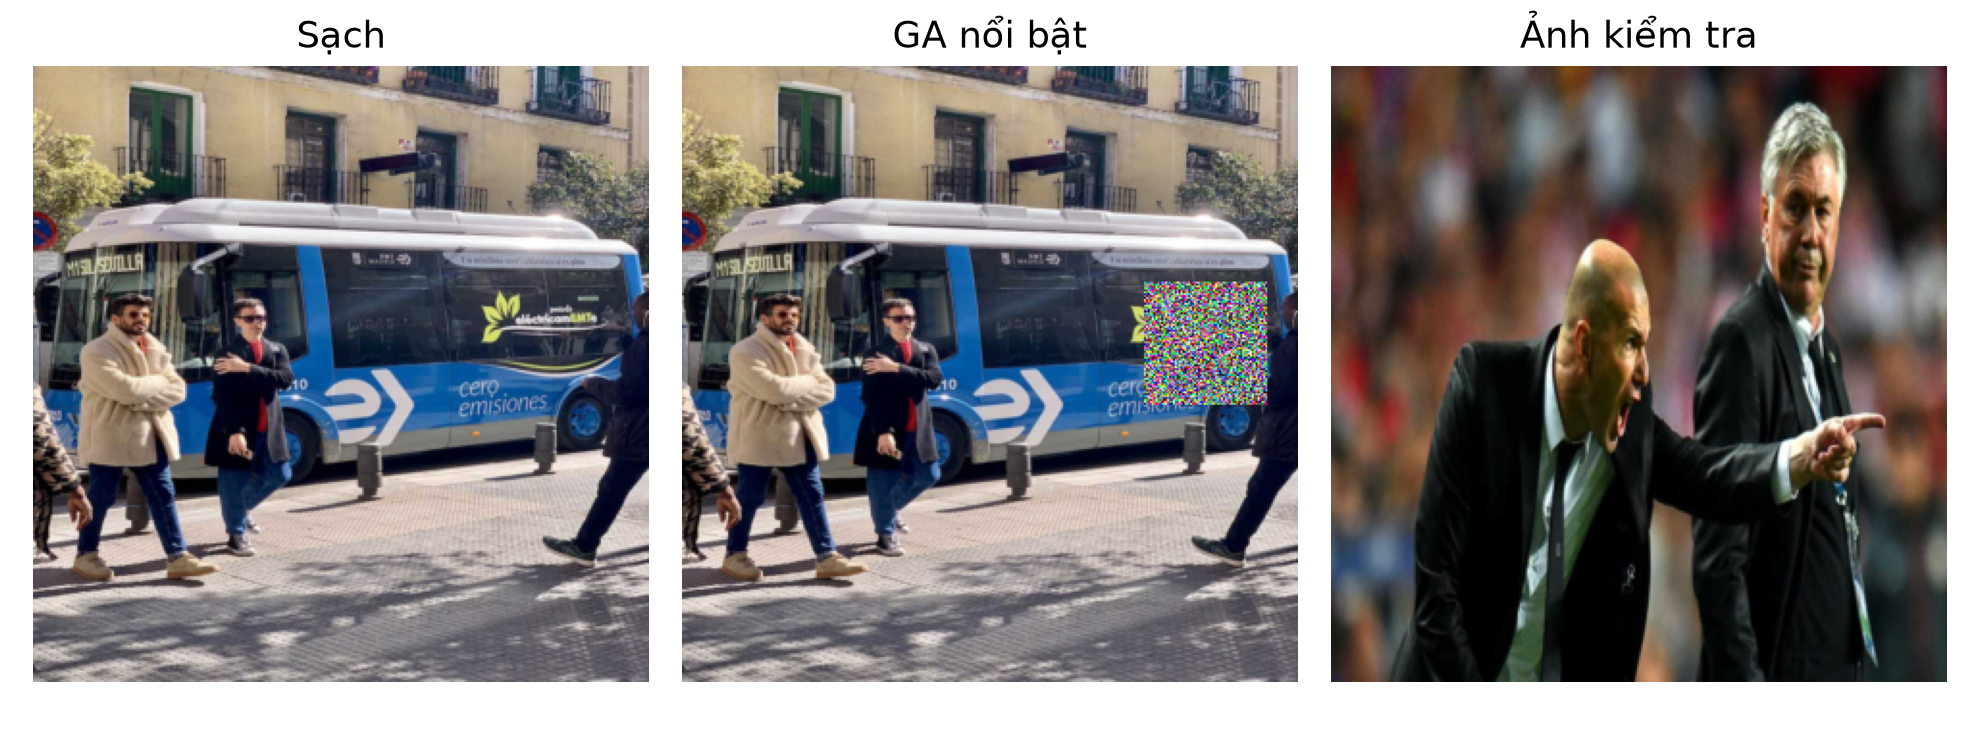
\includegraphics[width=0.88\textwidth]{outputs/local_q1_20261002_v2/image_examples.png}
\caption{Ảnh đầu vào của phép kiểm chứng cục bộ: ảnh tối ưu sạch, ảnh chèn miếng dán SG-GA seed 0 và ảnh kiểm tra khác nội dung. Miếng dán có kích thước 64×64 trên ảnh 320×320 (4\% diện tích); không vẽ hộp phát hiện trong hình này. Hai ảnh nguồn là ảnh ví dụ đi kèm Ultralytics; đây là chèn số, không phải miếng dán đã in.}
\label{fig:examples}
\end{figure*}

Hình~\ref{fig:examples} minh họa đúng ảnh được đưa vào mô hình sau co kích thước; ảnh kiểm tra không được dùng để tiến hóa miếng dán.

Phép đo riêng NMS dùng 10 seed sinh hộp khác nhau cho mỗi mức $N$, năm lượt khởi động và 20 lượt đo trên cùng bộ hộp. Trung vị 20 lượt tạo một quan sát seed. Kích thước hộp và mức chồng lấn cũng ảnh hưởng thời gian; các điểm $N=3.000$ hoặc 8.400 là tải tổng hợp trực tiếp, không phải số dự đoán của mô hình 320.

\subsection{Kiểm chứng bổ sung trên dữ liệu có nhãn}

COCO128 gồm 128 ảnh đầu của COCO train2017 và nhãn hộp định dạng YOLO, tải từ nguồn Ultralytics \cite{coco128}. Tập này có thể trùng dữ liệu huấn luyện của trọng số; nó chỉ được dùng để chẩn đoán hậu xử lý và đánh đổi phòng thủ, không để xác lập khả năng khái quát trên tập kiểm tra độc lập. Miếng dán seed 0 được quy định trước, không chọn theo kết quả COCO128 và không tối ưu lại trên tập này. Ba phương pháp và các họa tiết đối chứng giữ vị trí từ ảnh tối ưu; ảnh sạch là đối chứng ghép cặp theo ảnh.

Phép kiểm chứng này bổ sung ô bàn cờ đúng nghĩa với ô 4×4 pixel, bên cạnh sọc chéo của lượt hai ảnh, nhiễu đều và màu xám. Tổng cộng có tám điều kiện và ba cấu hình hậu xử lý. Kiểm tra trực tiếp tệp ZIP nguồn ghi nhận ảnh 250 và 508 không có tệp nhãn; nhãn 656 và 659 không có ảnh tương ứng. Cả 128 ảnh được giữ lại; hai ảnh thiếu nhãn được xử lý với tập nhãn rỗng theo quy ước của mã nạp Ultralytics, không tự bổ sung nhãn. Bản kê cấu hình lưu danh mục ngoại lệ này; AP là giá trị chẩn đoán phụ thuộc bộ nhãn đã cung cấp.

Mỗi điều kiện trên từng ảnh có một lượt suy luận khởi động và ba lượt đo. Dự đoán được lưu đệm để so sánh ba cấu hình ngưỡng/giới hạn trên cùng đầu ra. Mỗi cấu hình hậu xử lý có hai lượt khởi động và năm lượt đo; trung vị thời gian là quan sát ở mức ảnh. Suy luận và hậu xử lý được đo riêng nên không suy ra FPS toàn trình bằng cách cộng các trung vị. Thứ tự điều kiện và cấu hình được xáo trộn; mọi điều kiện dùng cùng bộ ảnh, kích thước, NMS và trọng số.

Độ chính xác và độ bao phủ được tính gộp các hộp tại IoU 0,5, ghép hộp dự đoán theo điểm giảm dần với hộp nhãn cùng lớp, mỗi nhãn chỉ ghép một lần. AP chẩn đoán dùng nội suy 101 mức độ bao phủ và trung bình các lớp có nhãn; mAP chẩn đoán tiếp tục lấy trung bình tại IoU từ 0,50 đến 0,95, bước 0,05. Đây không phải mAP COCO chính thức: bộ nhãn không có thông tin đối tượng đám đông/bỏ qua, phép ghép và NMS không phải trình đánh giá COCO chuẩn, và AP phụ thuộc ngưỡng lọc được báo. Bốn kiểm tra đơn vị xác nhận hộp khớp chính xác, sai lớp, phát hiện giả đứng trước hộp đúng và hộp trùng lặp.

\section{Kết quả}

\subsection{Kiểm chứng chiều fitness}

Mã nguồn dùng \texttt{max}, \texttt{argmax} và \texttt{topk}, do đó fitness càng lớn càng tốt. Điều này phù hợp với phương trình ở Mục 4.4. Bất kỳ bảng nào coi số fitness nhỏ hơn là tốt hơn đều sai và đã bị loại.

\subsection{Đo riêng thành phần NMS}

\begin{table}[ht]
\centering
\small
\caption{NMS torchvision đo trực tiếp trên máy cục bộ. Giá trị là trung bình ± độ lệch chuẩn giữa 10 seed hộp; mỗi seed dùng trung vị 20 lượt sau 5 lượt khởi động. Hộp được sinh trực tiếp, không phải đầu ra của mô hình phát hiện.}
\begin{tabular}{rrr}
\toprule
$N$ & Số cặp lý thuyết & Độ trễ (ms) \\
\midrule
50 & 1.225 & $0{,}071\pm0{,}052$ \\
100 & 4.950 & $0{,}064\pm0{,}044$ \\
500 & 124.750 & $0{,}550\pm0{,}354$ \\
1.000 & 499.500 & $1{,}838\pm0{,}582$ \\
2.100 & 2.203.950 & $5{,}514\pm2{,}758$ \\
3.000 & 4.498.500 & $9{,}953\pm2{,}752$ \\
8.400 & 35.275.800 & $70{,}363\pm15{,}055$ \\
\bottomrule
\end{tabular}
\label{tab:nmsbench}
\end{table}

Từ 50 lên 3.000 hộp, số cặp lý thuyết tăng $3.672{,}24\times$, trong khi tỷ lệ hai độ trễ trung bình khoảng $141{,}1\times$. Đây là tỷ số hai trung bình, không phải trung bình tỷ số ghép cặp. Mức 50 và 100 hộp không tăng đơn điệu do thời gian quá ngắn và độ phân tán lớn. Bảng~\ref{tab:nmsbench} và Hình~\ref{fig:nms} mô tả triển khai torchvision trên một máy; chúng không xác lập độ trễ của mã NMS thuần PyTorch trong đường ống phát hiện hay một máy chủ biên khác. Phép đo cũ 0,415/23,647 ms không có bản kê cấu hình nên không được gộp vào kết quả mới.

\begin{figure*}[t]
\centering
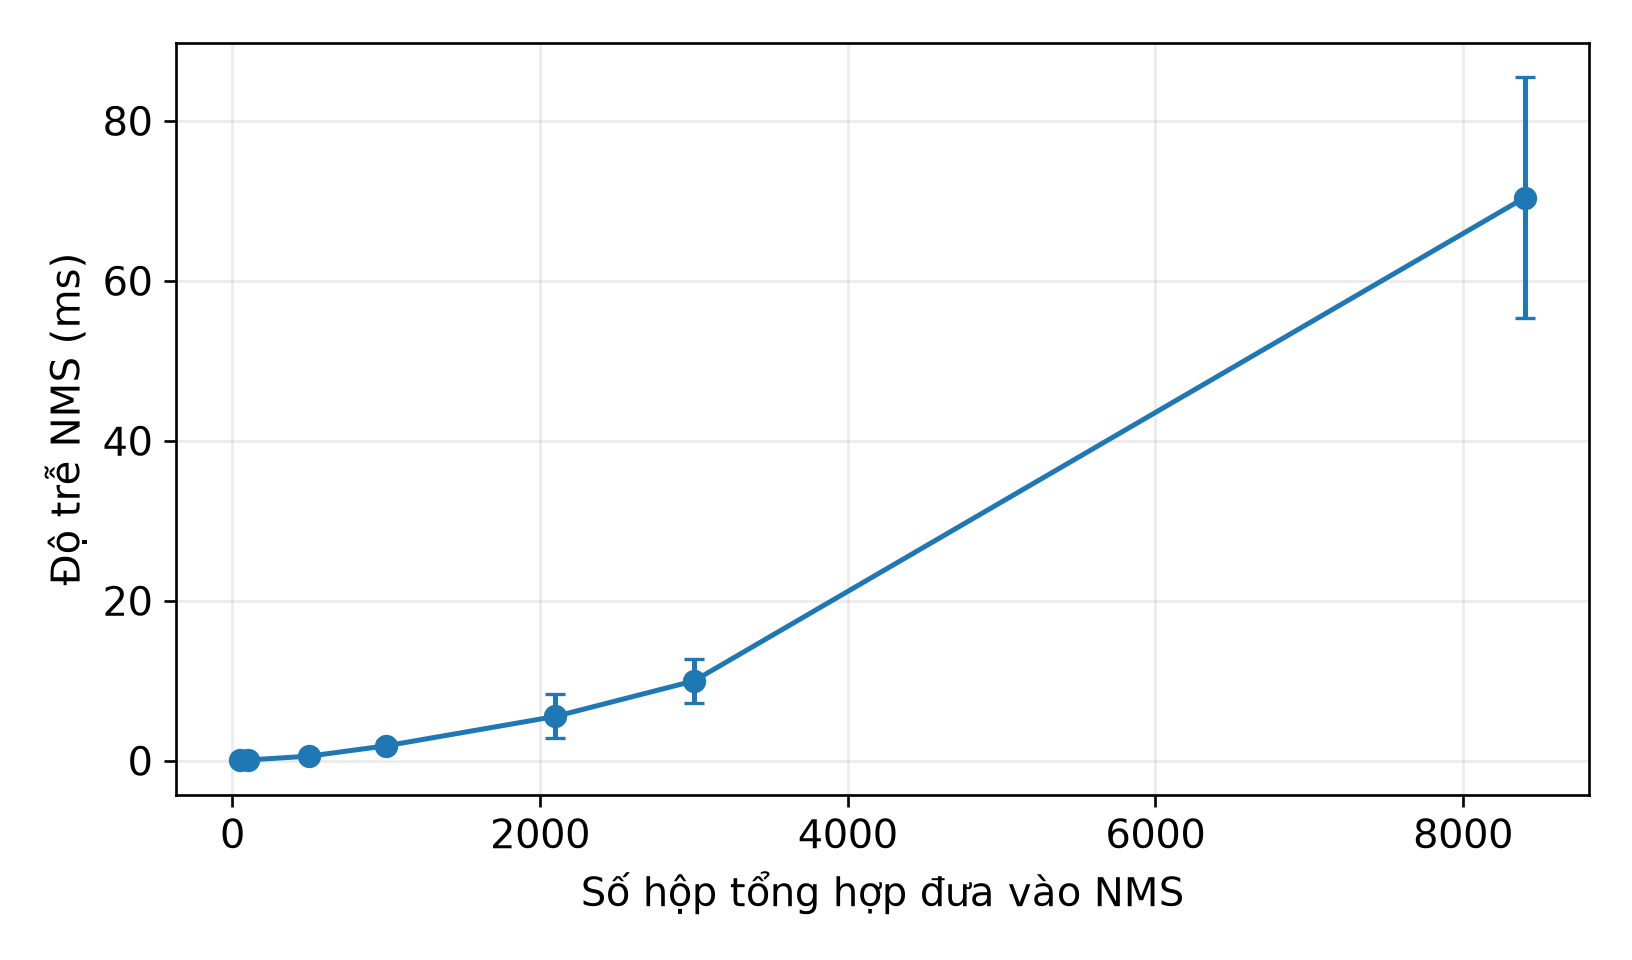
\includegraphics[width=0.72\textwidth]{outputs/local_q1_20261002_v2/figures_corrected/nms_local.png}
\caption{Độ trễ NMS torchvision theo số hộp tổng hợp trên CPU i5-1335U. Điểm và thanh sai số là trung bình và độ lệch chuẩn của trung vị thời gian giữa 10 seed hộp. Các mức 3.000 và 8.400 không phải số ứng viên do miếng dán tạo ra.}
\label{fig:nms}
\end{figure*}

\subsection{So sánh tối ưu cùng ngân sách trên ảnh tự nhiên}

\begin{table*}[t]
\centering
\caption{Kết quả tối ưu trên ảnh bus, 10 seed, cùng 400 truy vấn ảnh mỗi seed. Giá trị là trung bình ± độ lệch chuẩn giữa seed. Fitness là cực đại điểm EOT đã quan sát, không phải kỳ vọng EOT được kiểm tra độc lập.}
\begin{tabularx}{\textwidth}{Xrrr}
\toprule
Phương pháp & Fitness tốt nhất & Truy vấn/seed & Thời gian tối ưu (s) \\
\midrule
GA vị trí nổi bật & $312{,}61\pm10{,}65$ & 400 & $81{,}84\pm28{,}41$ \\
GA vị trí trung tâm & $367{,}39\pm18{,}40$ & 400 & $95{,}12\pm26{,}03$ \\
Tìm kiếm ngẫu nhiên & $309{,}97\pm5{,}65$ & 400 & $92{,}09\pm33{,}82$ \\
\bottomrule
\end{tabularx}
\label{tab:optimizer_local}
\end{table*}

Bảng~\ref{tab:optimizer_local} cho thấy GA trung tâm đạt điểm cao hơn SG-GA trong cấu hình này. Chênh lệch SG-GA với tìm kiếm ngẫu nhiên chỉ khoảng 2,64 điểm; chưa có bằng chứng để coi quy tắc Laplacian là lựa chọn vị trí vượt trội. Hình~\ref{fig:convergence} thể hiện cực đại tích lũy theo truy vấn; đường tăng không tự chứng minh miếng dán gây tải cao hơn ảnh sạch vì điểm còn phụ thuộc biến đổi EOT của toàn ảnh.

Chênh lệch fitness ghép cặp SG-GA trừ GA trung tâm là $-54{,}78$, khoảng tin cậy thăm dò 95\% $[-66{,}81;-42{,}45]$. So với tìm kiếm ngẫu nhiên, chênh lệch là $2{,}64$, khoảng $[-1{,}92;7{,}64]$. Kết quả này chỉ mô tả 10 seed trên một ảnh tối ưu, không cho phép xếp hạng phương pháp trên một phân bố ảnh hay phần cứng khác.

\begin{figure*}[t]
\centering
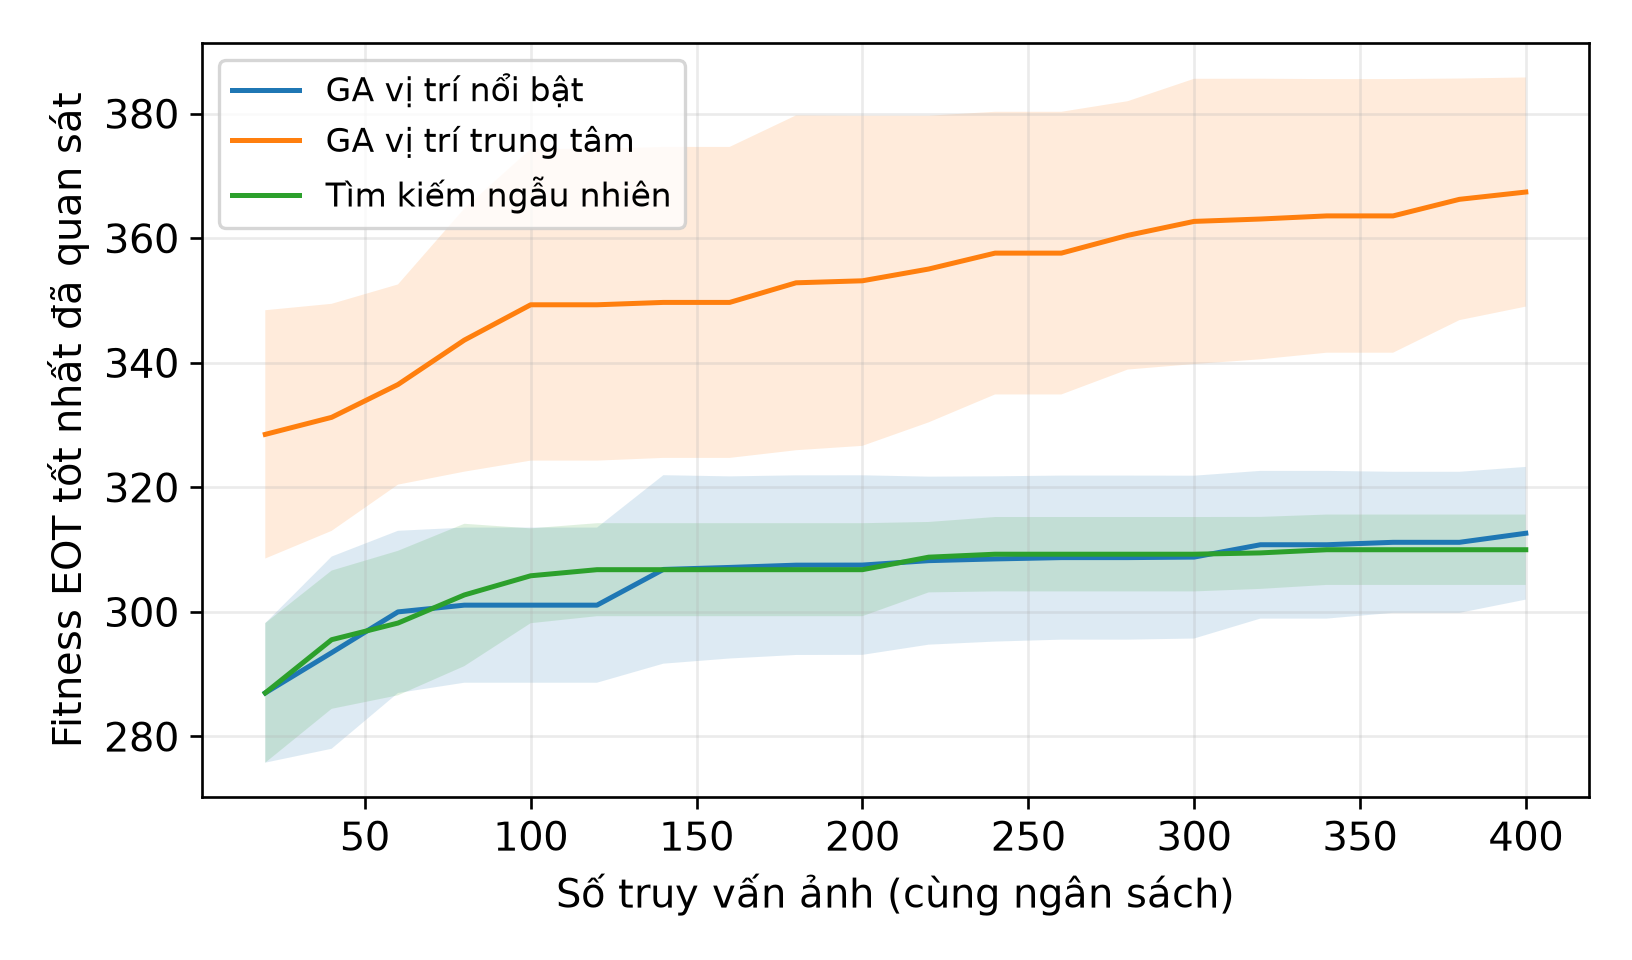
\includegraphics[width=0.72\textwidth]{outputs/local_q1_20261002_v2/figures_corrected/convergence_local.png}
\caption{Tiến trình tìm kiếm trên ảnh bus với cùng ngân sách 400 truy vấn. Đường là trung bình cực đại fitness EOT đã quan sát của 10 seed; vùng mờ là ± một độ lệch chuẩn giữa seed, không phải khoảng tin cậy. Mọi phương pháp đều tối đa hóa fitness.}
\label{fig:convergence}
\end{figure*}

\subsection{Ứng viên và chi phí thực thi trên hai ảnh tự nhiên}

\begin{table*}[t]
\centering
\small
\caption{Đánh giá không EOT tại ngưỡng 0,01, không giới hạn trước NMS. Trung bình ± độ lệch chuẩn giữa 10 seed; mỗi seed dùng trung vị năm lượt đo. Tổng thời gian chỉ gồm suy luận, lọc và NMS. Thông lượng là vòng xử lý ảnh tĩnh, không phải FPS camera.}
\begin{tabularx}{\textwidth}{Xlrrrrr}
\toprule
Điều kiện & Ảnh & Ứng viên & Phát hiện cuối & NMS (ms) & Tổng (ms) & Thông lượng (ảnh/s) \\
\midrule
Sạch & bus & 118,0 & 20,0 & $17{,}82\pm7{,}20$ & $267{,}4\pm122{,}5$ & $4{,}19\pm1{,}53$ \\
SG-GA & bus & $115{,}4\pm4{,}8$ & $20{,}0\pm1{,}1$ & $23{,}30\pm12{,}87$ & $316{,}1\pm164{,}6$ & $3{,}63\pm1{,}86$ \\
GA trung tâm & bus & $134{,}8\pm2{,}7$ & $23{,}4\pm1{,}3$ & $20{,}64\pm6{,}46$ & $268{,}8\pm101{,}1$ & $4{,}03\pm1{,}41$ \\
Sạch & zidane & 122,0 & 20,0 & $18{,}30\pm5{,}84$ & $251{,}6\pm69{,}0$ & $4{,}21\pm1{,}25$ \\
SG-GA & zidane & $119{,}1\pm3{,}5$ & $17{,}7\pm1{,}1$ & $14{,}45\pm5{,}96$ & $242{,}0\pm97{,}7$ & $4{,}46\pm1{,}26$ \\
GA trung tâm & zidane & $135{,}9\pm6{,}9$ & $21{,}1\pm0{,}7$ & $21{,}97\pm9{,}90$ & $285{,}5\pm120{,}5$ & $3{,}81\pm1{,}48$ \\
\bottomrule
\end{tabularx}
\label{tab:pipeline_local}
\end{table*}

SG-GA không khuếch đại số ứng viên ở ngưỡng 0,01 trên cả hai ảnh (Bảng~\ref{tab:pipeline_local}). Tỷ số độ trễ NMS trung bình so với ảnh sạch là khoảng 1,31 trên bus nhưng 0,79 trên zidane; tỷ số tổng thời gian tương ứng là 1,18 và 0,96. Độ phân tán thời gian lớn, nên không quy toàn bộ chênh lệch cho miếng dán. Mức CPU tiến trình chuẩn hóa toàn máy của ảnh sạch và SG-GA trên bus là $12{,}23\pm2{,}81$\% và $11{,}46\pm4{,}86$\%; trên zidane là $12{,}73\pm2{,}59$\% và $12{,}89\pm2{,}67$\%. Các giá trị này không cho thấy cạn kiệt CPU. RSS biến thiên lớn theo thời điểm đo và không được dùng để khẳng định rò rỉ hay cạn kiệt bộ nhớ.

\begin{figure*}[t]
\centering
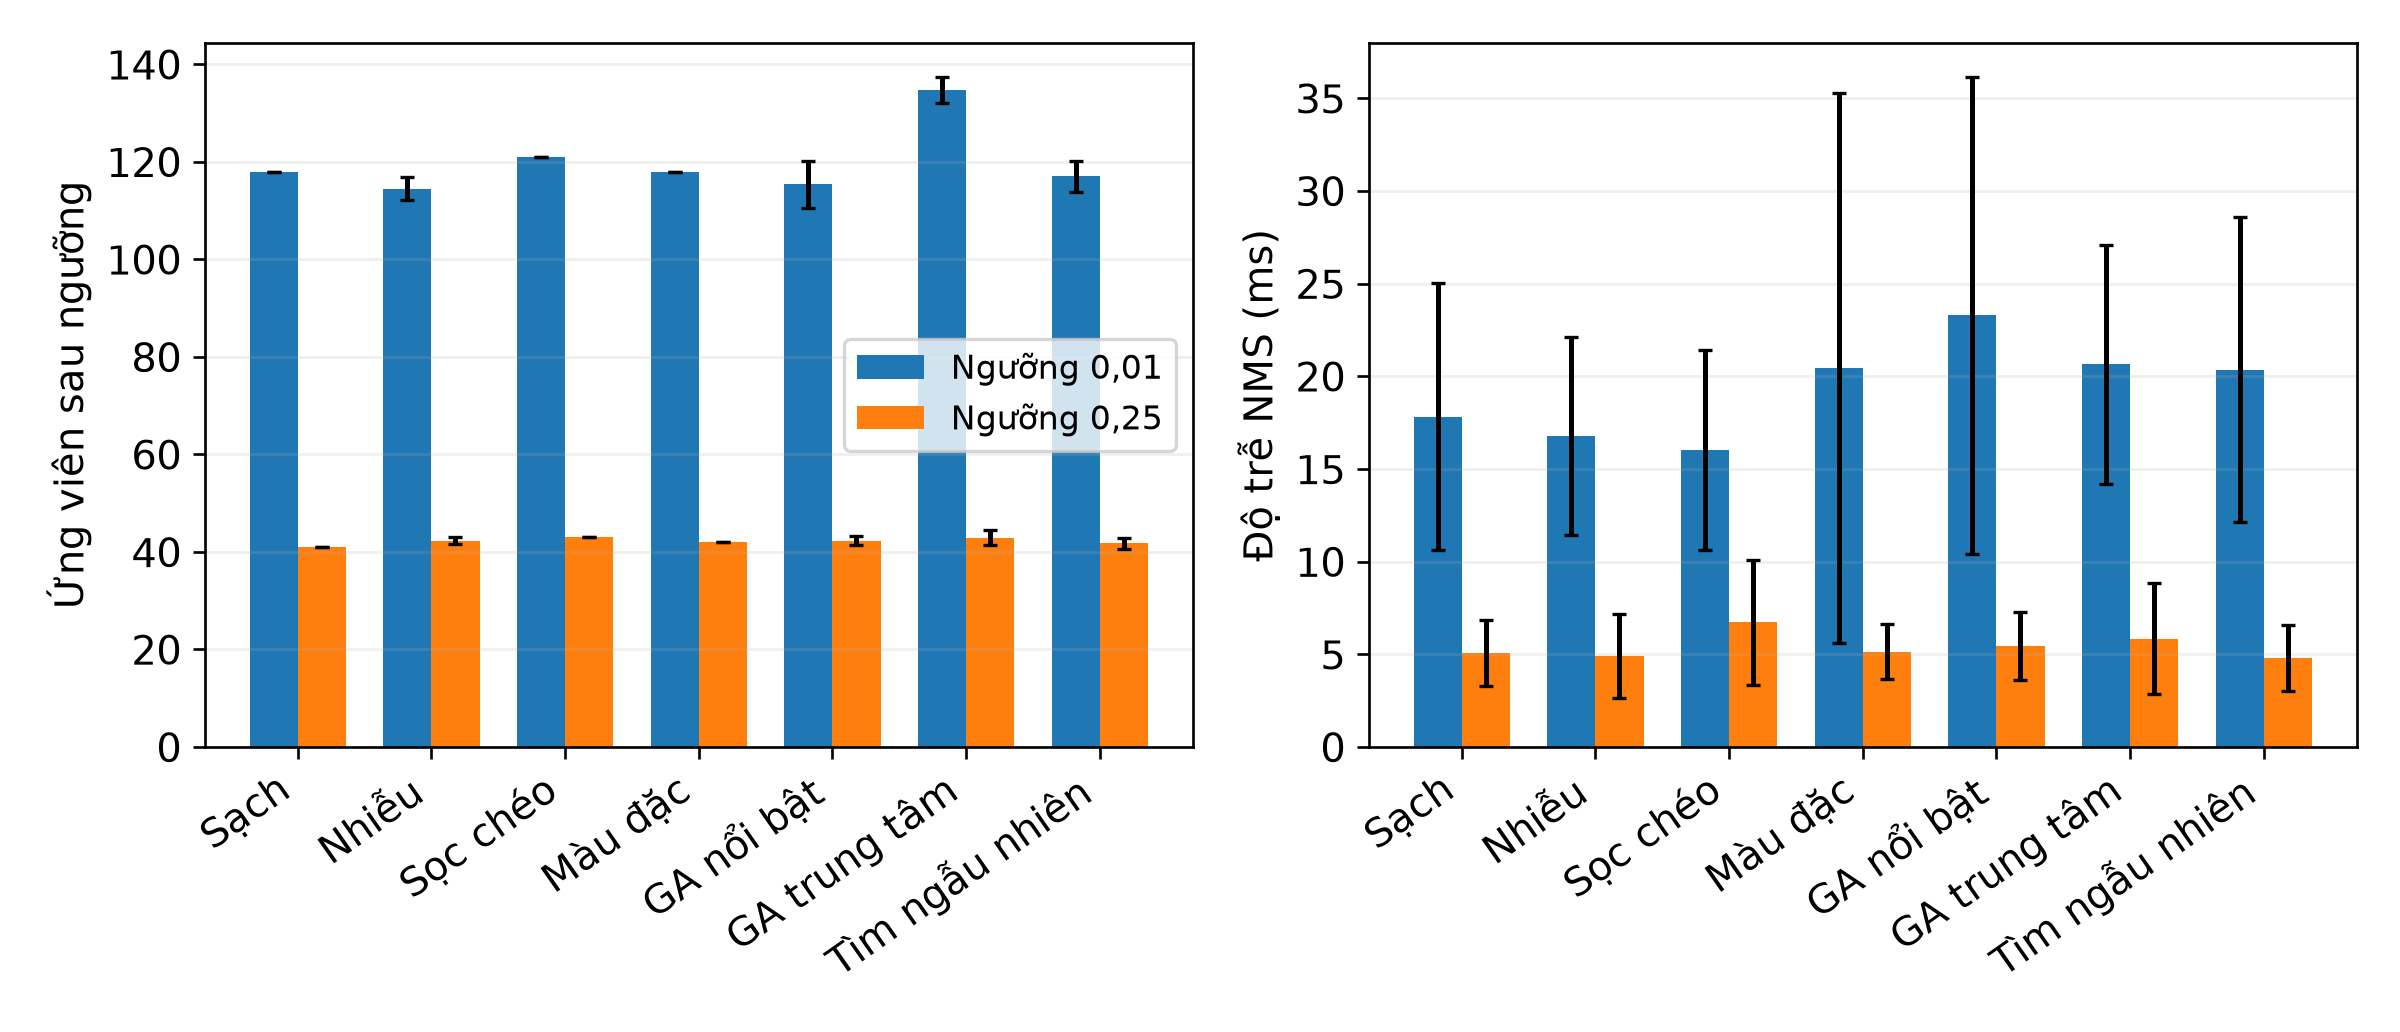
\includegraphics[width=0.95\textwidth]{outputs/local_q1_20261002_v2/figures_corrected/candidates_latency_bus.png}
\caption{Ứng viên sau ngưỡng và độ trễ NMS thuần PyTorch trên ảnh bus, không giới hạn trước NMS, tại hai ngưỡng đánh giá. Cột và thanh sai số là trung bình ± độ lệch chuẩn giữa 10 seed. Nhiễu và các họa tiết là đối chứng cùng diện tích; sọc chéo là tên đúng của trường checkerboard trong dữ liệu thô.}
\label{fig:bus}
\end{figure*}

\begin{figure*}[t]
\centering
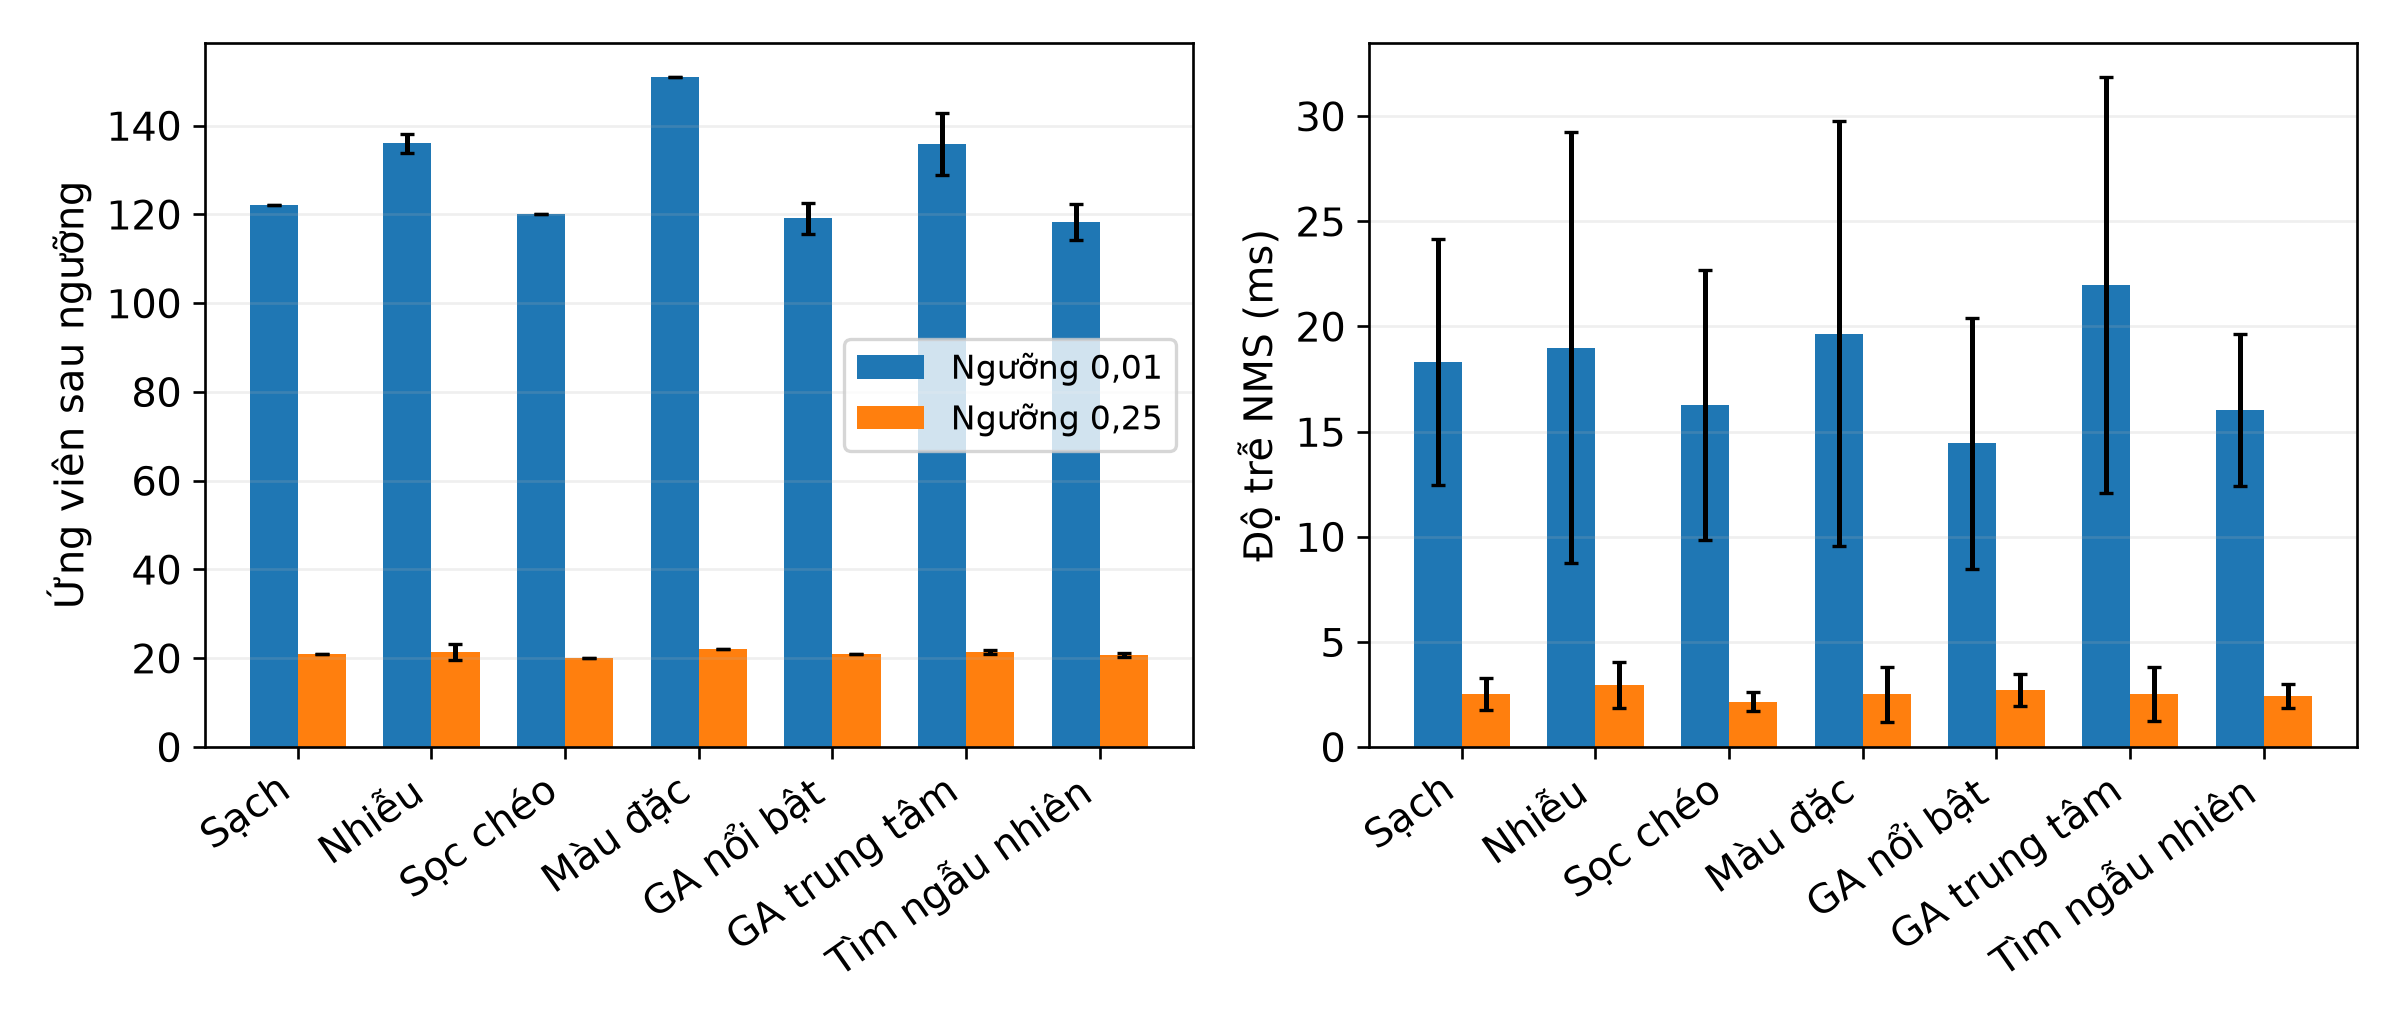
\includegraphics[width=0.95\textwidth]{outputs/local_q1_20261002_v2/figures_corrected/candidates_latency_zidane.png}
\caption{Ứng viên sau ngưỡng và độ trễ NMS trên ảnh zidane, không dùng ảnh này để tối ưu miếng dán. Cột và thanh sai số là trung bình ± độ lệch chuẩn giữa 10 seed. Các miếng dán tối ưu giữ vị trí từ bus; họa tiết đối chứng được chọn lại vị trí Laplacian, nên so sánh họa tiết ở đây có yếu tố nhiễu do vị trí.}
\label{fig:zidane}
\end{figure*}

Hình~\ref{fig:bus} và Hình~\ref{fig:zidane} cho thấy ngưỡng 0,25 làm số ứng viên giảm mạnh ở mọi điều kiện. Trên bus, SG-GA có $42{,}3\pm0{,}9$ ứng viên so với 41 của ảnh sạch; trên zidane, cả hai có 21 ứng viên. Việc tăng nhẹ ứng viên trên một ảnh không xác lập suy giảm dịch vụ; chưa có thời hạn hay tiêu chí thành công DoS được thiết kế trước. Độ chính xác của giới hạn ứng viên cần đánh giá trên dữ liệu có nhãn.

Ở ngưỡng 0,01, khoảng tin cậy thăm dò 95\% của chênh lệch tổng thời gian SG-GA trừ ảnh sạch là $[-34{,}43;154{,}16]$ ms trên bus và $[-56{,}35;30{,}89]$ ms trên zidane. Cả hai đều bao gồm không; không có bằng chứng nhất quán về tăng thời gian toàn vòng xử lý. Đây không phải bằng chứng tương đương hai điều kiện hay bảo đảm hệ thống miễn nhiễm.

\subsection{Ứng viên và độ chính xác trên COCO128}

Phép chạy hoàn tất 3.072 bản ghi, trên 128 ảnh, tám điều kiện và ba cấu hình. Bộ nhãn dùng 929 hộp thuộc 71 lớp. Tại ngưỡng 0,01 không giới hạn trước NMS, SG-GA seed 0 có trung bình 114,78 ứng viên so với 116,06 của ảnh sạch; chênh lệch ghép cặp là $-1{,}28$, khoảng tin cậy thăm dò 95\% $[-5{,}21;2{,}16]$ ứng viên. Chênh lệch NMS trung bình là $-0{,}452$ ms, khoảng $[-0{,}920;-0{,}031]$ ms; không diễn giải phân tích hậu nghiệm này thành chứng minh phòng thủ phổ quát. Kết quả không hỗ trợ khuếch đại tải NMS bởi miếng dán SG-GA đã chọn trên tập này.

\begin{table*}[t]
\centering
\small
\caption{Khối lượng hậu xử lý trên COCO128, 128 ảnh ghép cặp, miếng dán SG-GA seed 0. Hai cột đếm là trung bình giữa ảnh; thời gian NMS là trung vị [Q1; Q3] của các trung vị năm lượt đo từng ảnh. Ứng viên được đếm trước giới hạn; đầu vào NMS được đếm sau giới hạn.}
\begin{tabularx}{\textwidth}{XXrrX}
\toprule
Điều kiện & Cấu hình & Ứng viên & Vào NMS & NMS (ms) [Q1; Q3] \\
\midrule
Sạch & Ngưỡng 0,01 & 116,06 & 116,06 & 5,12 [2,55; 10,88] \\
Sạch & Ngưỡng 0,25 & 23,27 & 23,27 & 1,19 [0,77; 1,84] \\
Sạch & 0,01 + top-100 & 116,06 & 70,31 & 4,51 [2,38; 6,60] \\
SG-GA & Ngưỡng 0,01 & 114,78 & 114,78 & 5,08 [2,70; 10,77] \\
SG-GA & Ngưỡng 0,25 & 21,74 & 21,74 & 1,17 [0,69; 1,71] \\
SG-GA & 0,01 + top-100 & 114,78 & 72,29 & 4,65 [2,56; 6,63] \\
\bottomrule
\end{tabularx}
\label{tab:coco_latency}
\end{table*}

\begin{table*}[t]
\centering
\small
\caption{Độ chính xác chẩn đoán trên cùng 128 ảnh, 929 hộp nhãn. P/R là độ chính xác/độ bao phủ gộp tại IoU 0,5; AP50/mAP dùng nội suy 101 mức và trung bình lớp tại IoU 0,5/0,5--0,95. Tất cả cột chỉ số dùng \%. Đây không phải kết quả mAP COCO chính thức; ngưỡng lọc và NMS không phân biệt lớp được giữ rõ trong từng hàng.}
\begin{tabularx}{\textwidth}{XXrrrr}
\toprule
Điều kiện & Cấu hình & P (\%) & R (\%) & AP50 (\%) & mAP (\%) \\
\midrule
Sạch & Ngưỡng 0,01 & 22,45 & 55,11 & 46,00 & 32,74 \\
Sạch & Ngưỡng 0,25 & 78,93 & 35,09 & 34,66 & 26,89 \\
Sạch & 0,01 + top-100 & 33,33 & 49,19 & 44,71 & 32,17 \\
SG-GA & Ngưỡng 0,01 & 22,19 & 52,85 & 41,70 & 29,82 \\
SG-GA & Ngưỡng 0,25 & 77,40 & 32,08 & 30,98 & 23,96 \\
SG-GA & 0,01 + top-100 & 31,78 & 47,58 & 40,43 & 29,34 \\
\bottomrule
\end{tabularx}
\label{tab:coco_accuracy}
\end{table*}

Bảng~\ref{tab:coco_latency} và Bảng~\ref{tab:coco_accuracy} phân biệt chi phí hậu xử lý với chất lượng phát hiện. Ở ngưỡng 0,01, AP50 chẩn đoán giảm từ 46,00\% xuống 41,70\% khi chèn SG-GA, trong khi số ứng viên và thời gian NMS không tăng. Điều này là suy giảm tính toàn vẹn của phát hiện trong phép thử, không phải bằng chứng tấn công tính sẵn sàng. Hình~\ref{fig:coco} giữ đầy đủ các phương pháp và họa tiết đối chứng; các miếng dán khác cũng làm giảm độ bao phủ ở mức độ tương tự.

\begin{figure*}[t]
\centering
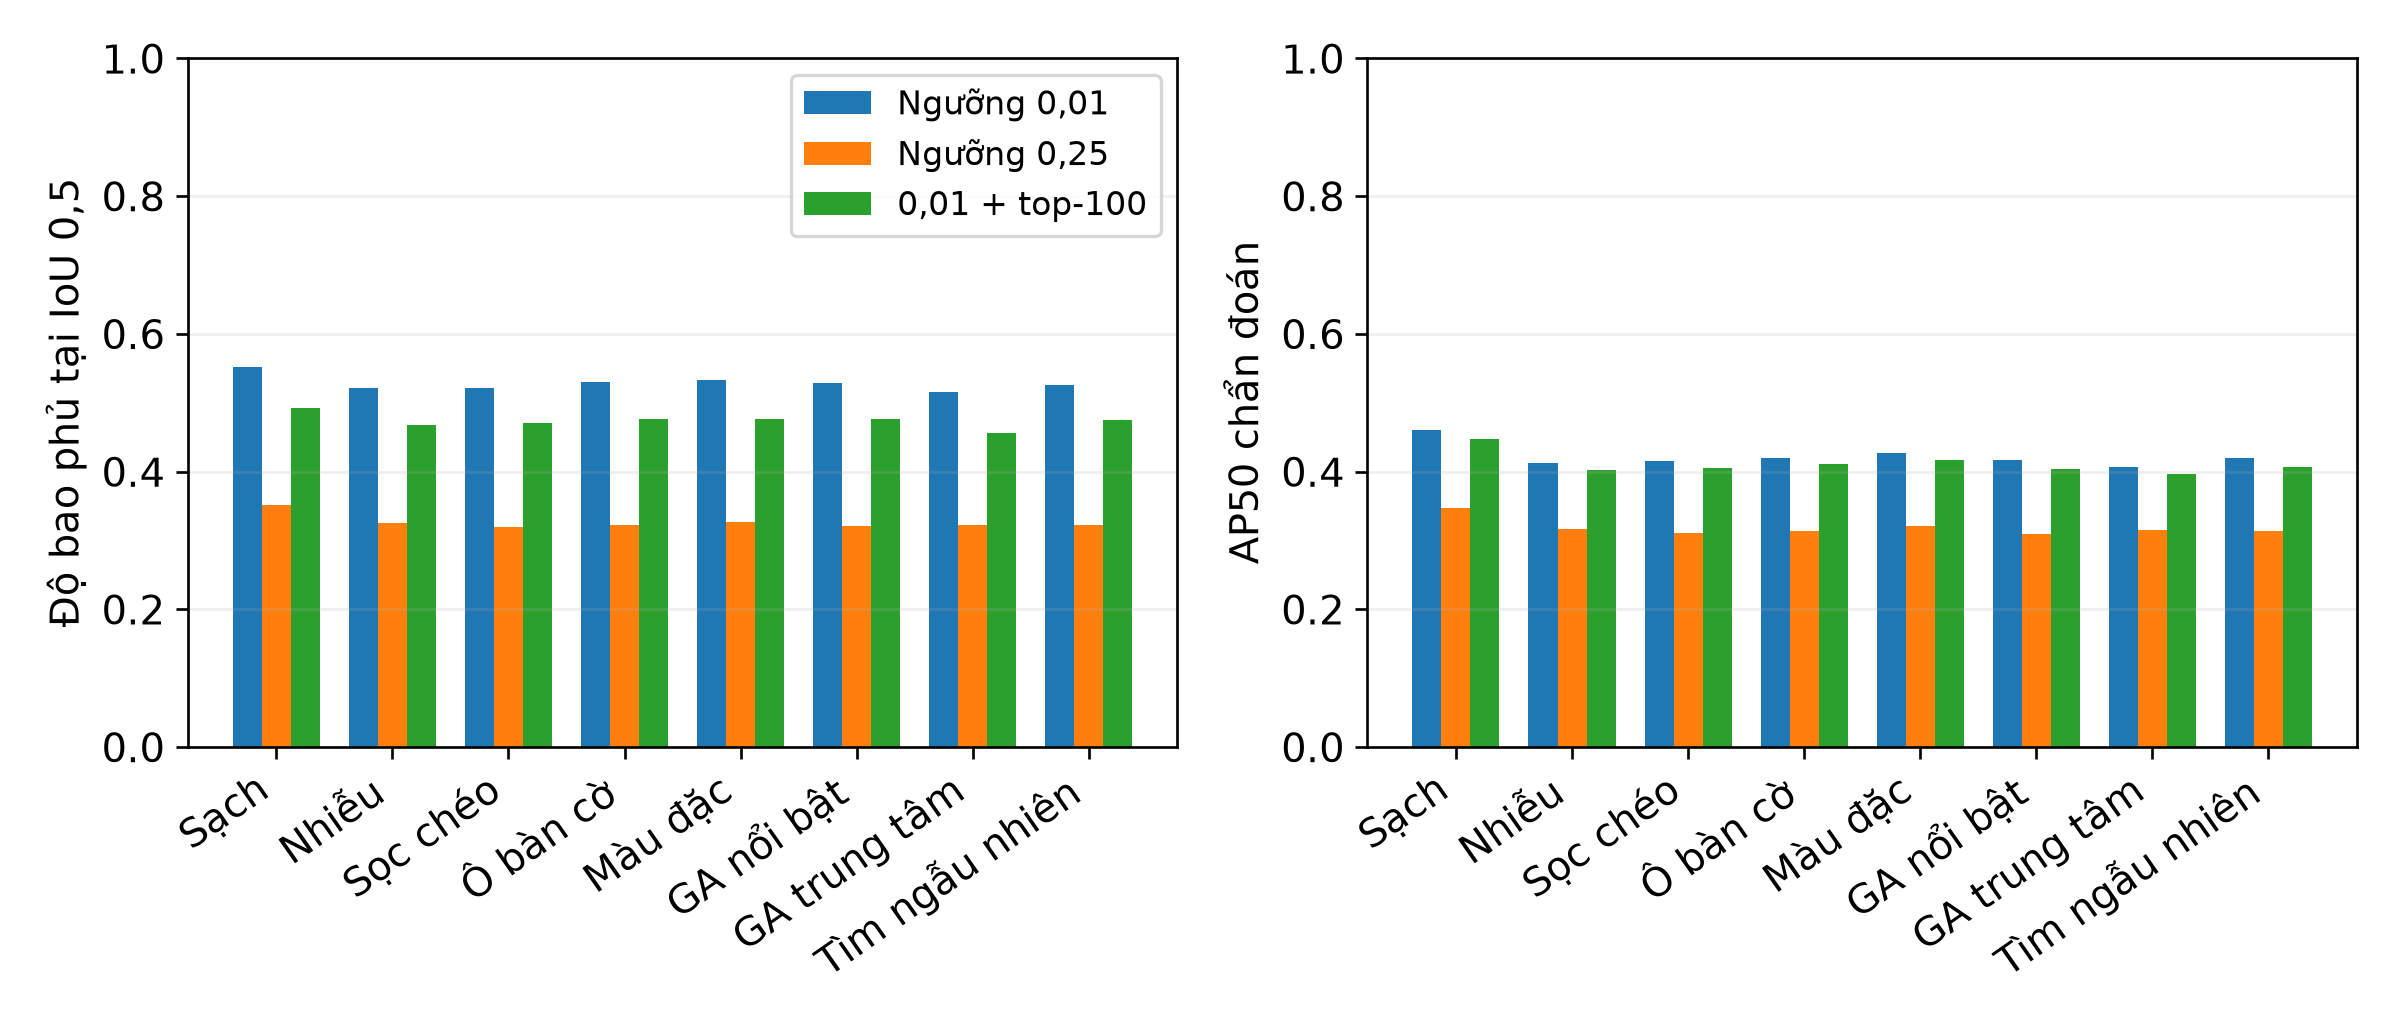
\includegraphics[width=0.95\textwidth]{outputs/local_coco128_20261002/figures_corrected/accuracy_defense.png}
\caption{Độ bao phủ và AP50 chẩn đoán trên 128 ảnh COCO128 cho tám điều kiện và ba cấu hình hậu xử lý. Các chỉ số có thang 0--1; AP được tính gộp bộ ảnh, không phải trung bình AP từng ảnh. Mỗi phương pháp dùng miếng dán seed 0 cố định và cùng bộ nhãn; không có thanh sai số vì không đánh giá phân bố miếng dán theo seed trong lượt này.}
\label{fig:coco}
\end{figure*}

\subsection{Kết quả tối ưu lưu trước đây}

\begin{table*}[t]
\centering
\caption{Tóm tắt đầu ra 10 seed hiện có. Độ lệch chuẩn được tính giữa seed. Kết quả dùng tensor ảnh nền ngẫu nhiên và chỉ mang tính thăm dò.}
\begin{tabularx}{\textwidth}{Xrrr}
\toprule
Phương pháp & Fitness tốt nhất & Thế hệ kết thúc & Độ phân tán cuối \\
\midrule
GA hướng dẫn bởi độ nổi bật & $65{,}07\pm4{,}67$ & $15{,}4\pm3{,}81$ & $13{,}49\pm3{,}13$ \\
GA không dùng độ nổi bật & $64{,}02\pm5{,}17$ & $14{,}7\pm2{,}26$ & $14{,}99\pm2{,}55$ \\
Tìm kiếm ngẫu nhiên & $15{,}18\pm0{,}51$ & -- & -- \\
\bottomrule
\end{tabularx}
\label{tab:optimizer}
\end{table*}

Chênh lệch fitness tốt nhất giữa hai GA là khoảng 1,05 điểm, nhỏ hơn độ lệch chuẩn trong từng nhóm. Lượt chạy tìm kiếm ngẫu nhiên cũ dùng 500 lượt đánh giá/seed, trong khi GA cho phép tối đa 600 lượt đánh giá và áp dụng EOT khác. Bảng~\ref{tab:optimizer} chỉ mô tả các kết quả lưu trước đây; phép so sánh cùng ngân sách trong các lượt kiểm chứng mới được báo cáo riêng.

\subsection{Cảnh tổng hợp và ứng viên phát hiện}

\texttt{proper\_dos\_sim.py} dùng cảnh tạo bằng OpenCV, ngưỡng tin cậy 0,001 và hai luồng CPU. Số ứng viên sau ngưỡng trung bình là 47,3 trên ảnh sạch, 55,7 khi chèn miếng dán số và 53,4 trên ảnh suy giảm bằng EOT; cực đại lần lượt là 95, 118 và 105. Điều kiện được đặt tên “physical” trong chương trình cũ thực chất làm mờ, thêm nhiễu và thay đổi màu trong phần mềm. Vì vậy điều kiện này được gọi là mô phỏng suy giảm ảnh trong bài.

Kết quả này không hỗ trợ kết luận mô hình phát hiện tạo trên 3.000 ứng viên sau ngưỡng. Giá trị $N=3.000$ trong phép đo riêng NMS là số hộp tổng hợp được tạo trực tiếp. Cấu hình 320 hiện chỉ có 2.100 vị trí dự đoán trước lọc.

\subsection{Nhật ký camera và hệ thống}

Hai cặp nhật ký ảnh sạch/miếng dán số gồm 60 và 100 khung hình không cho thấy hiệu ứng CPU nhất quán. Ở cặp 60 khung hình, CPU trung bình là 76,57\% trên ảnh sạch và 76,70\% khi chèn miếng dán; ở cặp 100 khung hình, mức tải khi chèn miếng dán thấp hơn ảnh sạch, 19,95\% so với 28,68\%. Thời gian NMS trung bình gần bằng nhau trong từng cặp. Thiếu thứ tự điều kiện ngẫu nhiên, thông tin khởi động và cấu hình máy khiến các nhật ký này chưa đủ cho suy luận nhân quả.

\section{Thực nghiệm loại bỏ thành phần và phân tích độ nhạy}

\subsection{Thực nghiệm theo kích thước miếng dán}

\begin{table*}[t]
\centering
\caption{Thực nghiệm theo kích thước miếng dán hiện có; mỗi mức chỉ là một lượt chạy, nên không dùng để kết luận xu hướng.}
\begin{tabularx}{\textwidth}{XXXX}
\toprule
Diện tích mục tiêu & Miếng dán (px) & Diện tích thực & Fitness tốt nhất \\
\midrule
1\% & 32 & 1,00\% & 63,45 \\
2\% & 45 & 1,98\% & 64,47 \\
4\% & 64 & 4,00\% & 63,82 \\
8\% & 90 & 7,91\% & 66,76 \\
16\% & 128 & 16,00\% & 62,15 \\
\bottomrule
\end{tabularx}
\label{tab:patch_area}
\end{table*}

Fitness không tăng đơn điệu theo diện tích. Một lượt chạy ở mỗi mức chưa tách được tính ngẫu nhiên của thuật toán khỏi ảnh hưởng kích thước. Thực nghiệm theo diện tích cần ít nhất 10 seed mỗi mức, cùng tập ảnh và ngân sách truy vấn; kết quả phải gồm số ứng viên và độ trễ thực đo bên cạnh fitness.

\subsection{Họa tiết đối chứng và kết quả âm}

Ở ngưỡng tin cậy 0,25 trên ảnh nền ngẫu nhiên trong kết quả cũ, miếng dán Sponge tạo trung bình 8,65 ứng viên và độ trễ NMS 1,34 ms. Màu đặc đạt 20,6 ứng viên/2,71 ms; ô bàn cờ đạt 16,2 ứng viên/2,74 ms. Miếng dán tối ưu không vượt các họa tiết đơn giản trong quy trình này. Kết quả âm gợi ý cần kiểm tra sự phù hợp của ảnh tối ưu, ngưỡng tối ưu và ngưỡng triển khai.

\newexperiment{mở rộng đối chứng trên tập ảnh tự nhiên cố định, gồm nhiễu Gaussian, họa tiết tương tự mã QR, miếng dán tấn công tính toàn vẹn và ít nhất một tấn công tăng độ trễ NMS đã công bố; giữ cùng phần cứng, diện tích và ngân sách truy vấn.}

\subsection{Độ nhạy theo ngưỡng tin cậy}

Đầu ra đánh giá phòng thủ hiện dùng ảnh nền ngẫu nhiên. Ở $\tau=0,01$ ghi nhận 10 ứng viên; từ $\tau=0,05$ trở lên là 0. Kết quả cho thấy độ nhạy cao với ngưỡng nhưng không thể dùng để đánh giá đánh đổi giữa phòng thủ và độ chính xác vì không có ảnh và nhãn phát hiện chuẩn. Cần đo mAP/precision/recall trên dữ liệu có nhãn.

\section{Đánh giá tính chuyển giao}

Kết quả thăm dò cũ ghi nhận tỷ lệ độ trễ 1,173 cho YOLOv8n, 1,002 cho Faster R-CNN, 0,929 cho RetinaNet và 1,012 cho DETR. Mã bao YOLO chỉ đo suy luận trước NMS, còn các mô hình torchvision gộp hậu xử lý vào lượt suy luận. Các tỷ lệ vì vậy không cùng đại lượng đo và không xác lập khả năng chuyển giao giữa kiến trúc.

Kết luận đúng ở trạng thái hiện tại là: \emph{tính chuyển giao chưa được xác lập}. Không có bằng chứng hỗ trợ các số 2.150+/1.800+ ứng viên hoặc phần trăm CPU/FPS trong bảng cũ.

\newexperiment{chuẩn hóa tiền xử lý, kích thước đầu vào, khởi động, đồng bộ hóa và ranh giới đo trên YOLO, SSD/Faster R-CNN/RetinaNet cùng DETR/RT-DETR; đánh giá nhiều miếng dán và seed trên cùng ảnh tự nhiên.}

\section{Đánh giá thế giới vật lý}

Không có tệp dữ liệu và mã đủ để tái tạo thực nghiệm với miếng dán đã in. EOT và hàm \texttt{degrade\_patch\_physical} chỉ là mô phỏng. Vì vậy nghiên cứu hiện chỉ hỗ trợ \emph{giả thuyết sơ bộ về chuyển đổi từ môi trường số sang vật lý}, không hỗ trợ kết luận DoS vật lý.

Quy trình vật lý cần ghi vật liệu, máy in hoặc thiết bị hiển thị, kích thước cm, diện tích trong khung hình, mẫu camera, độ phân giải/FPS, bộ mã hóa, khoảng cách, ba góc quay, độ sáng và số phép thử. Thứ tự điều kiện phải được xáo trộn. Các đại lượng đo gồm $N_{\mathrm{active}}$, độ trễ NMS, độ trễ toàn trình, FPS, số lần trễ hạn và CPU/RSS của tiến trình. Mức tải CPU đơn lẻ không xác định thành công của tấn công.

\newexperiment{thử ít nhất $3\times3\times3\times2$ cấu hình khoảng cách, góc, mức sáng và camera/bộ mã hóa; $\geq10$ khối thử nghiệm mỗi điều kiện; dùng ảnh sạch, nhiễu ngẫu nhiên, ô bàn cờ và miếng dán tối ưu làm đối chứng.}

\section{Thảo luận}

\subsection{Ý nghĩa của kết quả hiện tại}

Phép đo riêng NMS xác nhận chi phí hậu xử lý tăng khi số hộp đầu vào tăng. Đánh giá miếng dán trong ảnh phải xác định liệu chính miếng dán có tạo thêm ứng viên và gây ảnh hưởng toàn trình hay không. Khoảng cách giữa khả năng gây tải bằng hộp tổng hợp và khả năng tạo các hộp đó qua ảnh là vấn đề thực nghiệm cốt lõi; phép đo riêng NMS không tự chứng minh DoS của hệ thống.

\subsection{Vai trò của độ nổi bật}

Phương sai Laplacian chọn vùng có cấu trúc ảnh mạnh, không trực tiếp đo độ nhạy của mô hình phát hiện. Vai trò của lựa chọn vị trí phải được đánh giá trên cùng ảnh nền, cùng seed và ngân sách truy vấn. Đường cong fitness tốt nhất đã quan sát cho thấy tiến triển tìm kiếm, nhưng điểm được chọn từ một mẫu EOT có thể phản ánh cả biến đổi ngẫu nhiên của toàn ảnh.

\subsection{Ngưỡng 0,01 và tính công bằng}

Ngưỡng thấp giúp phân biệt fitness giữa các cá thể nhưng có thể xa cấu hình triển khai. Bài báo báo riêng $\tau_{\mathrm{opt}}=0,01$ và ngưỡng đánh giá. Một miếng dán được tối ưu tại 0,01 phải được đo lại tại 0,25 để đánh giá hiệu lực khi đổi ngưỡng. Nếu hệ thống thực sự triển khai ở 0,01, ảnh sạch và độ chính xác cũng phải được đo ở ngưỡng đó.

\subsection{Kích thước miếng dán}

$64\times64$ trên $320\times320$ tương ứng 4\% diện tích. Nếu miếng dán được tăng độ phân giải lên khung hình $1280\times720$, phải định nghĩa phép biến đổi sao cho tỷ lệ diện tích hoặc góc quan sát được kiểm soát. $256\times256$ trên $1280\times720$ là khoảng 7,11\%, không phải mặc định 15--20\%. Không nên so trực tiếp kích thước pixel giữa hai độ phân giải.

\section{Hàm ý phòng thủ}

Giới hạn top-$k$ trước NMS và tăng ngưỡng đã được kiểm tra chẩn đoán trong cấu hình cục bộ. Giám sát số ứng viên tăng đột biến, điều tiết tải ngược hoặc bỏ khung hình và chuyển sang kiến trúc không dùng NMS vẫn là các đề xuất chưa được xác nhận trong phép kiểm chứng này.

Tham số \texttt{max\_det} trong mã cũ cắt danh sách sau khi NMS trả chỉ số, nên không giảm số ứng viên phải xử lý. Phép kiểm chứng mới áp dụng top-100 theo điểm tin cậy trước khi gọi NMS, rồi mới giới hạn 300 phát hiện đầu ra. Giới hạn trước NMS cần được đánh giá đồng thời về độ trễ và độ chính xác, đặc biệt khả năng tìm đủ đối tượng trong cảnh đông người.

Trên COCO128, với miếng dán SG-GA, top-100 giảm trung vị NMS từ khoảng 5,08 xuống 4,65 ms nhưng độ bao phủ giảm từ 52,85\% xuống 47,58\%, mất 5,27 điểm phần trăm. Tăng ngưỡng từ 0,01 lên 0,25 giảm trung vị NMS xuống 1,17 ms nhưng độ bao phủ còn 32,08\%. Ảnh sạch cũng chịu đánh đổi: độ bao phủ giảm từ 55,11\% xuống 49,19\% khi giới hạn top-100. Do vậy, việc lọc bớt hộp không được gọi là phòng thủ giữ nguyên độ chính xác. Các số này điều kiện trên bộ nhãn và NMS không phân biệt lớp đã mô tả, không phải cam kết hiệu năng triển khai.

\newexperiment{mở rộng quét ngưỡng/giới hạn ứng viên, điều tiết tải ngược thích nghi và đánh giá COCO chính thức trên tập kiểm tra độc lập; báo độ trễ/FPS, tỷ lệ trễ hạn cùng độ chính xác dưới cả ảnh sạch và các tấn công mạnh.}

\section{Hạn chế và các mối đe dọa tới tính hợp lệ}

\subsection{Tính hợp lệ nội tại}

Điều phối hệ điều hành, tiến trình nền, thay đổi tần số và việc thu hình có thể ảnh hưởng CPU/FPS. Lượt kiểm chứng mới có khởi động và xáo trộn thứ tự điều kiện, nhưng máy cá nhân vẫn chạy các tác vụ khác và chưa cô lập hoàn toàn tiến trình. CPU được tính từ thời gian CPU của tiến trình chia cho thời gian thực thi; mức chuẩn hóa toàn máy tiếp tục chia cho 12 bộ xử lý logic. Mẫu đo ngắn có thể chịu lượng tử hóa của đồng hồ CPU.

\subsection{Tính hợp lệ cấu trúc}

$N_{\mathrm{active}}$ đại diện cho khối lượng công việc NMS; mức tải CPU không đồng nghĩa DoS. FPS có thể giảm do suy luận, giải mã, dựng hình hoặc thu hình. Thành công của tấn công cần dựa trên độ trễ, vi phạm thời hạn và thông lượng cùng phép đo theo công đoạn. FPS trong phép kiểm chứng ảnh tĩnh chỉ là thông lượng vòng lặp suy luận, không phải FPS camera.

\subsection{Tính hợp lệ bên ngoài}

Mô hình tối ưu và đánh giá cục bộ là YOLOv8n. Hai ảnh ví dụ và COCO128 giúp kiểm tra trên nội dung tự nhiên nhưng không đại diện phân bố camera thực tế. COCO128 thuộc train2017, có thể đã được dùng trong tiền huấn luyện; hai ảnh không có tệp nhãn được giữ theo quy ước nhãn rỗng. Một máy và một kiến trúc không hỗ trợ kết luận phổ quát về máy chủ biên. Co ảnh không giữ tỷ lệ và NMS không phân biệt lớp khác cấu hình triển khai Ultralytics tiêu chuẩn.

\subsection{Tính hợp lệ kết luận thống kê}

Các lượt mới dùng 10 seed trên cùng ảnh và ngân sách; các kết quả cũ dùng ảnh ngẫu nhiên vẫn được phân loại riêng. Seed, ảnh và lượt đo lặp không được gộp thành một cỡ mẫu duy nhất. Khoảng tin cậy bootstrap là thăm dò hậu nghiệm, không điều chỉnh đa so sánh và không thay cho kiểm định xác nhận giả thuyết được thiết kế trước. COCO128 dùng một miếng dán mỗi phương pháp, nên biến thiên giữa ảnh không ước lượng biến thiên của quần thể miếng dán. AP được tính gộp bộ ảnh, chưa có khoảng tin cậy.

\subsection{Tính hợp lệ vật lý}

Chưa có ma trận khoảng cách, góc, ánh sáng, vật liệu và camera. Mô phỏng suy giảm bằng EOT không định lượng đầy đủ quang học camera, dải màu máy in, chói sáng và nén ảnh thực.

\subsection{Tính hợp lệ của mã triển khai}

NMS thuần PyTorch của mã bao, NMS của torchvision, hậu xử lý Ultralytics và các mô hình không dùng NMS có hành vi khác nhau. Phép đo riêng hộp tổng hợp dùng torchvision; đánh giá hai ảnh dùng NMS không phân biệt lớp của mã bao. Các tỷ lệ độ trễ giữa hai phép đo không được xem là cùng một đường ống. Bản kê cấu hình lưu phiên bản đang nạp và mã băm nguồn để tái lập đúng triển khai.

\section{Cân nhắc đạo đức}

Nghiên cứu kiểm thử độ bền của hệ thống AI tại biên trên thiết bị thuộc quyền kiểm soát của nhóm. Các tệp công bố ưu tiên khả năng tái lập và biện pháp giảm thiểu. Phép kiểm chứng cục bộ giới hạn luồng, số truy vấn và kích thước hộp; không tác động lên hệ thống giám sát bên ngoài. Các giới hạn của giả định thông số nội bộ và bằng chứng vật lý được công bố để xác định phạm vi kết luận.

\section{Kết luận}

Bài báo kiểm chứng một khung tối ưu miếng dán hộp xám dựa trên điểm trước NMS, đồng thời tách mục tiêu đại diện khỏi chi phí hệ thống. Với 10 seed và 400 truy vấn mỗi phương pháp trên ảnh bus, SG-GA có fitness thấp hơn GA trung tâm và không có ưu thế rõ so với tìm kiếm ngẫu nhiên. Khi đo lại không EOT, SG-GA không làm tăng số ứng viên ở ngưỡng 0,01 trên hai ảnh ví dụ; độ trễ toàn vòng xử lý không tăng nhất quán. Trên COCO128, miếng dán seed 0 làm AP50 chẩn đoán giảm nhưng không khuếch đại số ứng viên hoặc chi phí NMS. Các kết quả này phân biệt suy giảm độ chính xác với tấn công tính sẵn sàng.

Phép đo riêng trên hộp tổng hợp xác nhận độ trễ NMS phụ thuộc tải đầu vào trong triển khai được đo, nhưng không chứng minh miếng dán tạo ra tải đó. Giới hạn top-100 và tăng ngưỡng giảm công việc hậu xử lý với chi phí giảm độ bao phủ, kể cả trên ảnh sạch. Kết quả hiện tại hỗ trợ một nghiên cứu kiểm chứng có thể tái lập và làm rõ giới hạn của fitness dựa trên ứng viên, chưa xác lập DoS, chuyển giao giữa kiến trúc hoặc hiệu lực vật lý. Để hướng tới công bố Q1, cần tối ưu trên nhiều ảnh, đối chứng tấn công mạnh, nhiều kiến trúc/phần cứng, định nghĩa trước tiêu chí chất lượng dịch vụ và thử miếng dán đã in có kiểm soát. Các kết quả âm phải được giữ lại trong những đánh giá đó.

\section*{Tuyên bố về trạng thái bằng chứng}

Các số liệu được truy vết tới tệp dữ liệu trong kho mã nguồn. Kết quả mới có bản kê cấu hình và mã băm; kết quả cũ được gắn rõ là thăm dò hoặc tổng hợp khi thích hợp. Những con số của bản thảo cũ không truy vết được tới nhật ký/cấu hình đã bị loại. Không suy tạo giá trị $p$, khoảng tin cậy hoặc kết quả vật lý.

\begin{thebibliography}{99}

\bibitem{brown2017}
T. B. Brown, D. Mané, A. Roy, M. Abadi, and J. Gilmer,
``Adversarial Patch,'' arXiv:1712.09665, 2017.

\bibitem{athalye2018}
A. Athalye, L. Engstrom, A. Ilyas, and K. Kwok,
``Synthesizing Robust Adversarial Examples,'' in \emph{Proc. ICML}, 2018, pp. 284--293.

\bibitem{shumailov2021}
I. Shumailov, Y. Zhao, D. Bates, N. Papernot, R. Mullins, and R. Anderson,
``Sponge Examples: Energy-Latency Attacks on Neural Networks,'' in \emph{Proc. IEEE EuroS\&P}, 2021, pp. 212--231.

\bibitem{wang2021daedalus}
D. Wang, C. Li, S. Wen, Q.-L. Han, S. Nepal, X. Zhang, and Y. Xiang,
``Daedalus: Breaking Non-Maximum Suppression in Object Detection via Adversarial Examples,'' \emph{IEEE Transactions on Cybernetics}, vol. 52, no. 8, pp. 7427--7440, 2022.

\bibitem{shapira2023}
A. Shapira, A. Zolfi, L. Demetrio, B. Biggio, and A. Shabtai,
``Phantom Sponges: Exploiting Non-Maximum Suppression to Attack Deep Object Detectors,'' in \emph{Proc. WACV}, 2023, pp. 4571--4580.

\bibitem{chen2024overload}
E.-C. Chen, P.-Y. Chen, I.-H. Chung, and C.-R. Lee,
``Overload: Latency Attacks on Object Detection for Edge Devices,'' in \emph{Proc. CVPR}, 2024, pp. 24716--24725.

\bibitem{ma2024slowtrack}
C. Ma, N. Wang, Q. A. Chen, and C. Shen,
``SlowTrack: Increasing the Latency of Camera-Based Perception in Autonomous Driving Using Adversarial Examples,'' \emph{Proc. AAAI}, vol. 38, no. 5, pp. 4062--4070, 2024, doi: 10.1609/aaai.v38i5.28200.

\bibitem{wang2025defense}
T. Wang, Z. Wang, C. Wang, Y. Shu, R. Deng, P. Cheng, and J. Chen,
``Can't Slow Me Down: Learning Robust and Hardware-Adaptive Object Detectors against Latency Attacks for Edge Devices,'' in \emph{Proc. CVPR}, 2025, pp. 19230--19240.

\bibitem{monteuuis2025}
J.-P. Monteuuis, C. Chen, and J. Petit,
``Latency NMS Attacks: Is It Real Life or Is It Just Fantasy?,'' in \emph{Advances in Neural Information Processing Systems}, vol. 38, 2025, doi: 10.52202/085713-1289.

\bibitem{coco128}
Ultralytics, ``COCO128 Dataset,'' tài liệu trực tuyến, truy cập ngày 02/10/2026. \url{https://docs.ultralytics.com/datasets/detect/coco128/}.

\end{thebibliography}

\end{document}
